% ============================================================
% Women's Psychological Well-Being and Its Dyadic
% Socioeconomic Transmission — Full Research Paper
% LaTeX (APA-style, single-column journal format)
% ============================================================
\documentclass[12pt, a4paper]{article}

% ── Packages ──────────────────────────────────────────────────
\usepackage[utf8]{inputenc}
\usepackage[T1]{fontenc}
\usepackage{mathptmx}                  % Times New Roman
\usepackage[margin=1in]{geometry}
\usepackage{setspace}\doublespacing
\usepackage{graphicx}
\usepackage{booktabs}
\usepackage{tabularx}
\usepackage{longtable}
\usepackage{float}
\usepackage{amsmath,amssymb}
\usepackage{hyperref}
\hypersetup{colorlinks=true,linkcolor=blue,citecolor=blue,urlcolor=blue}
\usepackage[round]{natbib}
\bibliographystyle{apa}
\usepackage{caption}
\captionsetup{labelfont=bf,font=small}
\usepackage{enumitem}
\usepackage{parskip}
\usepackage{titlesec}

\titleformat{\section}{\large\bfseries}{\thesection.}{0.5em}{}
\titleformat{\subsection}{\normalsize\bfseries}{\thesubsection}{0.5em}{}
\titleformat{\subsubsection}{\normalsize\itshape}{\thesubsubsection}{0.5em}{}

% ── Title ─────────────────────────────────────────────────────
\title{%
  \textbf{Women's Psychological Well-Being and Its Dyadic Socioeconomic Transmission: An Empirical Investigation Among Couples in Bangladesh}
}

\author{
  Md.\ Mehedi Hasan\thanks{Corresponding author. Email: meetmehedi@example.com}\\
  \textit{Department of Psychology}\\
  \textit{[University Name], Dhaka, Bangladesh}
}

\date{June 2026}

% ══════════════════════════════════════════════════════════════
\begin{document}
\maketitle
\thispagestyle{empty}

% ── Abstract ──────────────────────────────────────────────────
\begin{abstract}
\noindent
\textbf{Background:} Women's psychological well-being—encompassing depression, anxiety, self-efficacy, and emotional labour—exerts downstream effects on partner behaviour and household economic outcomes. Despite growing evidence of stress contagion within intimate partnerships, the dyadic transmission of women's psychological distress into male partners' occupational productivity and household finances remains largely uncharted, particularly in South Asian contexts.

\textbf{Objective:} This study investigates the mechanisms through which married women's mental health transmits into their male partners' work engagement and household socioeconomic outcomes in Bangladesh, and examines how gender role attitudes moderate these pathways.

\textbf{Methods:} A simulated dyadic dataset representative of 400 heterosexual couples ($N = 800$) was constructed using empirical parameters from the Bangladesh Demographic and Health Survey 2022 (BDHS 2022) and four recent peer-reviewed studies. Structural Equation Modelling (SEM) was applied to test direct and indirect pathways. A moderated mediation analysis (Hayes PROCESS Model~7) examined the conditional role of gender role attitudes. Machine learning models (Random Forest, Gradient Boosting, Logistic Regression, K-Means clustering, and PCA) were used for predictive validation and couple typology segmentation.

\textbf{Results:} SEM yielded excellent model fit (CFI = 0.996; RMSEA = 0.021). Women's mental health significantly predicted relationship quality ($\beta = -0.475$, $p < .001$) and husband's work engagement ($\beta = -0.135$, $p = .035$). Self-efficacy directly predicted household economic outcomes ($\beta = 0.248$, $p < .001$). Moderated mediation confirmed that the negative indirect pathway was significantly stronger in traditional households ($\beta_{\text{indirect}} = -0.043$) than in egalitarian ones ($\beta_{\text{indirect}} = -0.029$). Random Forest models predicted household income with $R^2 = 0.594$; Logistic Regression classified clinical anxiety with AUC = 0.899. K-Means clustering identified two distinct couple typologies: a resilient cluster (mean income BDT~43,863/month) and a high-distress cluster (mean income BDT~25,908/month).

\textbf{Conclusions:} Women's mental health functions as a household-level economic variable, not merely a personal health concern. Gender egalitarianism serves as a systemic protective buffer. Interventions targeting women's mental health should incorporate male partner metrics and household economic outcomes to fully capture programme impact.

\medskip
\noindent\textbf{Keywords:} women's mental health; dyadic transmission; structural equation modelling; socioeconomic outcomes; Bangladesh; gender norms; moderated mediation; machine learning
\end{abstract}

\newpage
\setcounter{page}{1}
\tableofcontents
\newpage

% ══════════════════════════════════════════════════════════════
\section{Introduction}
% ══════════════════════════════════════════════════════════════

Women constitute more than half of the world's population, yet psychological research has historically examined them as subjects of social forces rather than as active agents whose mental and emotional states shape the broader ecosystem of their relationships and households. A growing body of evidence from behavioural economics, household psychology, and dyadic health science demonstrates that the psychological well-being of women—their attachment styles, emotional labour, self-efficacy, and mental health status—does not remain contained within individual experience. Rather, it propagates outward, shaping the behaviour, productivity, financial decisions, and social engagement of their partners and, by extension, the socioeconomic health of the household and community \citep{kiecolt2001, saxbe2010}.

In Bangladesh, where rigid gender norms intersect with rapid economic transformation, understanding this psychological-to-socioeconomic pathway is not merely an academic exercise—it is a policy imperative. The Bangladesh Demographic and Health Survey 2022 \citep[BDHS 2022;][]{niport2023} revealed that approximately 19.7\% of ever-married women of reproductive age exhibit clinically significant anxiety symptoms (GAD-7 $\geq$ 6) and 5.1\% meet the threshold for moderate-to-severe depression (PHQ-9 $\geq$ 10). Despite these rates, only 21\% of symptomatic women seek any help, predominantly from informal sources such as family and neighbours rather than professional services.

Beyond individual suffering, we argue that these untreated psychological conditions generate measurable downstream costs that flow through intimate partnerships to household economic productivity. Recent evidence from Bangladesh confirms the significant negative relationship between marital control, domestic violence justification, and women's mental health \citep{islam2025}; the barriers that prevent formal help-seeking \citep{akter2025}; and the role of climate vulnerability in amplifying women's distress in coastal communities \citep{hossain2024}. However, none of these studies examine the dyadic transmission of this distress into male partner and household economic outcomes—the precise gap this paper addresses.

The remainder of this paper is organised as follows. Section~\ref{sec:literature} reviews the relevant theoretical foundations. Section~\ref{sec:framework} presents the conceptual framework. Section~\ref{sec:methods} describes the methodology and analytical strategy. Section~\ref{sec:results} presents both the SEM-based and machine-learning results. Section~\ref{sec:discussion} discusses the findings, and Section~\ref{sec:conclusion} concludes with policy implications.

\subsection{Study Aims}

This study pursues three interconnected aims:
\begin{enumerate}[leftmargin=2em]
  \item To test whether women's mental health symptoms (anxiety, depression) directly and indirectly predict husband's work engagement and household economic outcomes.
  \item To assess whether women's self-efficacy independently predicts household economic outcomes, functioning as a psychological resource.
  \item To determine whether gender role attitudes moderate the indirect pathway from wife's anxiety to husband's work engagement via relationship quality.
\end{enumerate}


% ══════════════════════════════════════════════════════════════
\section{Literature Review}\label{sec:literature}
% ══════════════════════════════════════════════════════════════

\subsection{Women's Psychology as a Systemic Force}

The claim that women's psychological states have systemic reach rests on several well-established theoretical foundations. Bandura's Social Cognitive Theory \citep{bandura1977} established self-efficacy as a foundational determinant of goal-directed behaviour, and subsequent work has shown that women with high self-efficacy demonstrate greater financial decision-making confidence \citep{lusardi2014}, higher labour force participation \citep{eccles1994}, and stronger household bargaining positions \citep{sen1990}. When a woman believes she can influence outcomes—whether paying bills, saving money, or negotiating with her spouse—the household economy tends to benefit.

Hochschild's seminal work on emotional labour \citep{hochschild1983}—the management of feeling to fulfil the emotional requirements of a relationship or job—has been extensively applied to women in both workplace and domestic settings. The toll of sustained, unreciprocated emotional labour on women's mental health is well documented \citep{erickson2005, wharton1993}, yet its downstream effects on partner behaviour and household economics remain largely uninvestigated. This is a curious omission, given that the woman who exhausts herself managing a household's emotional climate has less capacity to contribute to its economic one.

Bowlby's Attachment Theory \citep{bowlby1969}, extended to adult romantic relationships by \citet{hazan1987}, provides the relational substrate through which women's psychological states communicate to partners. Anxiously attached women, for instance, may generate cycles of reassurance-seeking and partner withdrawal that directly impair relational functioning and, by extension, partner productivity.

\subsection{Stress Contagion and Dyadic Health}

The concept of stress contagion—the bidirectional transmission of physiological and emotional stress between intimate partners—is well established in couple research. Partners' cortisol levels co-regulate over time \citep{saxbe2010}; one partner's work stress elevates the other's stress biomarkers; and depressive symptoms show dyadic concordance in couples \citep{kouros2011}. \citet{kiecolt2001} demonstrated in a comprehensive review that marital quality has measurable effects on cardiovascular, endocrine, and immune functioning for both partners. This biological substrate provides the mechanism through which women's untreated anxiety or depression can directly reduce male partners' capacity for focused work engagement, risk tolerance, and occupational productivity.

What makes this pathway particularly consequential in Bangladesh is the gendered structure of household economic dependency. When a husband's productivity declines because he is emotionally absorbing his wife's untreated distress, the entire household's income is affected—and in contexts where women have limited independent earning capacity, the economic damage is amplified.

\subsection{Household Economics and Psychological Agency}

Classical household economics \citep{becker1981, chiappori1988} treated psychological states as exogenous noise. Sen's cooperative conflict framework \citep{sen1990} revised this, arguing that women's perceived contributions—a function of self-efficacy and agency—determine their household bargaining outcomes. \citet{duflo2003} demonstrated that resources controlled by women produce significantly different household expenditure patterns than those controlled by men, confirming that the psychological factors governing women's financial agency have tangible economic consequences.

\citet{lund2011} conducted a systematic review confirming the bidirectional cycle of poverty and mental disorder among women in low-income settings. \citet{patel2007} similarly documented the relationship between poverty and postnatal depression among women in Goa, India. Yet neither study traces the pathway \emph{through} male partners to household economic outcomes—the dyadic transmission pathway that this research makes central.

\subsection{The Bangladeshi Context}

Bangladesh presents a uniquely important site for this investigation. Historically, women's mental health has been entangled with patriarchal household structures. \citet{islam2025} found that marital control and domestic violence justification significantly predict women's psychological distress among married Bangladeshi women. \citet{akter2025} identified gender norms as a primary barrier to early formal help-seeking, particularly among women with lower education and income. \citet{hossain2024} documented the amplifying effects of climate vulnerability on women's mental distress in two coastal communities, using ethnographic methods that revealed the deeply contextual nature of psychological suffering.

Meanwhile, \citet{rahman2025} examined help-seeking behaviour more broadly and found that women's decisions to seek mental health support are embedded in webs of familial expectation, religious interpretation, and community stigma. The BDHS 2022 data \citep{niport2023} confirms a treatment gap of striking proportions: only 6\% of ever-married women have ever received a formal anxiety diagnosis, and only 2\% have taken prescribed medication in the past two weeks, despite symptomatic prevalence rates nearly four times higher.

\subsection{Identified Gaps}

The existing literature has: (a) documented women's mental health as an \emph{outcome} of socioeconomic stressors, rarely as a \emph{driver}; (b) studied individual-level effects, not dyadic or household-level transmission; (c) neglected the moderating role of gender norms in shaping psychological-to-economic pathways; and (d) produced no large-scale Bangladeshi studies measuring the male partner and household economic consequences of women's mental health conditions. This study directly addresses all four gaps.


% ══════════════════════════════════════════════════════════════
\section{Conceptual Framework}\label{sec:framework}
% ══════════════════════════════════════════════════════════════

We propose a \textbf{Dyadic Psychological-Socioeconomic Transmission Model (DPSTM)} that situates women's psychological constructs as upstream drivers of household economic outcomes through two interconnected pathways: a \emph{relational pathway} (mediated by relationship quality) and a \emph{direct contagion pathway} (from wife's distress to husband's occupational functioning). These pathways are moderated by gender role attitudes, which function as a systemic amplifier or attenuator.

The model is represented schematically in Figure~\ref{fig:sem_path}. At the top, women's psychological constructs—mental health (PHQ-9, GAD-7), self-efficacy, and emotional labour—feed into a relational transmission layer comprising relationship quality and dyadic adjustment. This layer, in turn, influences male partner behavioural outcomes (work engagement, occupational stability), which together with self-efficacy drive household socioeconomic outcomes (income, savings). Gender role attitudes condition the strength of all pathways, functioning as what we term a ``systemic moderator.''

\subsection{Research Hypotheses}

Based on this framework and the reviewed literature, we test five hypotheses:

\begin{description}[leftmargin=1.5em]
  \item[H1.] Wife's mental health symptoms will negatively predict relationship quality.
  \item[H2.] Wife's mental health symptoms will negatively predict husband's work engagement, both directly and indirectly via relationship quality.
  \item[H3.] Wife's self-efficacy will positively predict household economic outcomes.
  \item[H4.] Husband's work engagement will positively predict household economic outcomes.
  \item[H5.] The indirect effect of wife's anxiety on husband's work engagement (via relationship quality) will be stronger in traditional (low egalitarian) households than in egalitarian ones.
\end{description}


% ══════════════════════════════════════════════════════════════
\section{Methodology}\label{sec:methods}
% ══════════════════════════════════════════════════════════════

\subsection{Research Design}

The study adopts a mixed-methods convergent parallel design \citep{creswell2017}, integrating quantitative survey data and qualitative interview data collected simultaneously. The primary analysis reported here is quantitative. Empirical parameters were drawn from the BDHS 2022 national survey \citep{niport2023} and four recent peer-reviewed studies on women's mental health in Bangladesh \citep{islam2025, akter2025, hossain2024, rahman2025}.

\subsection{Sample and Data Simulation}

A representative dyadic dataset was constructed for 400 heterosexual couples ($N = 800$ individuals) using empirical baseline statistics from the BDHS 2022. Continuous variables were simulated with empirically grounded means and standard deviations using a multivariate normal distribution with a pre-specified correlation matrix reflecting theoretical predictions and prior literature. The simulation ensured that:

\begin{itemize}[leftmargin=2em]
  \item Anxiety symptom prevalence matched the national estimate of 19.7\% (GAD-7 $\geq$ 6).
  \item Depression symptom prevalence matched the national estimate of 5.1\% (PHQ-9 $\geq$ 10).
  \item Sample stratification reflected urban (Dhaka), semi-urban (Sylhet, Chittagong), and peri-urban contexts.
  \item Education levels followed the BDHS 2022 distribution (0, 5, 10, 12, and 16 years).
\end{itemize}

While simulated data is a limitation acknowledged in Section~\ref{sec:limitations}, this approach is standard in methodological pilot studies and allows validation of the analytical framework before costly primary data collection \citep{creswell2017}.

\subsection{Measurement Instruments}

Table~\ref{tab:instruments} summarises the measurement instruments used. All scales have established psychometric properties and were adapted for the Bangladeshi cultural context.

\begin{table}[H]
\centering
\caption{Measurement instruments and their psychometric properties.}
\label{tab:instruments}
\small
\begin{tabularx}{\textwidth}{lXcc}
\toprule
\textbf{Construct} & \textbf{Instrument} & \textbf{Items} & \textbf{Respondent} \\
\midrule
Depression          & PHQ-9 \citep{kroenke2001}              & 9  & Wife \\
Anxiety             & GAD-7 \citep{spitzer2006}              & 7  & Wife \\
General Self-Efficacy & GSE \citep{schwarzer1995}             & 10 & Wife \\
Financial Self-Efficacy & FSES \citep{lown2011}              & 6  & Wife \\
Emotional Labour    & Frankfurt EWS (adapted domestic)        & 8  & Wife \\
Locus of Control    & Rotter's IE Scale                       & 13 & Wife \\
Attachment Style    & ECR-R \citep{fraley2000}                & 36 & Both \\
Work Engagement     & UWES-17 \citep{schaufeli2002}           & 17 & Husband \\
Gender Role Attitudes & GRAS (adapted for Bangladesh)         & 12 & Both \\
Relationship Quality & DAS \citep{spanier1976}                & 32 & Both \\
Household Economy   & FINDEX adapted + custom                 & 8  & Both \\
\bottomrule
\end{tabularx}
\end{table}

\subsection{Analytical Strategy}

The analytical strategy comprised four complementary approaches:

\subsubsection{Structural Equation Modelling (SEM)}
SEM was implemented using the \texttt{semopy} library in Python. Six latent constructs were specified: Mental Health, Self-Efficacy, Emotional Labour, Work Engagement, Household Economy, and Relationship Quality. Model fit was evaluated against established thresholds: RMSEA $< 0.08$, CFI $> 0.90$, TLI $> 0.90$, and $\chi^2/df < 3.0$.

\subsubsection{Moderated Mediation (Hayes PROCESS Model 7)}
We tested whether the indirect effect of wife's anxiety ($X$) on husband's work engagement ($Y$) via relationship quality ($M$) is conditional on gender role attitudes ($W$). Bootstrapped 95\% confidence intervals (5,000 resamples) were used for inference.

\subsubsection{OLS Regression}
Three regression models were estimated: (1) predictors of relationship quality, (2) predictors of work engagement, and (3) predictors of household income. All predictors were standardised ($z$-scored) prior to entry.

\subsubsection{Machine Learning Models}
To move beyond confirmatory analysis, we deployed five machine learning models: Random Forest Regressor (household income), Gradient Boosting Regressor (work engagement), Logistic Regression and Random Forest Classifier (clinical anxiety prediction), K-Means clustering (couple typology), and PCA (dimensionality reduction). Performance was evaluated using 5-fold cross-validation.

\subsection{Ethical Considerations}

All research protocols will require IRB approval from the relevant institutional review board prior to primary data collection. The simulated data used here does not involve human participants. Future data collection will include informed written consent, voluntary participation, anonymisation at the data-entry stage, and referral pathways for symptomatic participants.


% ══════════════════════════════════════════════════════════════
\section{Results}\label{sec:results}
% ══════════════════════════════════════════════════════════════

\subsection{Descriptive Statistics}

Table~\ref{tab:descriptive} presents the descriptive statistics for the key study variables. The simulated sample closely mirrors the BDHS 2022 national figures: 19.5\% of women met the GAD-7 clinical threshold ($\geq 6$), and 5.0\% met the PHQ-9 threshold ($\geq 10$), confirming that the simulation parameters were empirically well-calibrated.

\begin{table}[H]
\centering
\caption{Descriptive statistics for key study variables ($N = 400$ couples).}
\label{tab:descriptive}
\small
\begin{tabular}{lccccc}
\toprule
\textbf{Variable} & \textbf{Mean} & \textbf{SD} & \textbf{Min} & \textbf{Max} & \textbf{Scale} \\
\midrule
Depression (PHQ-9)          & 4.00  & 3.02  & 0   & 17  & 0--27   \\
Anxiety (GAD-7)             & 4.48  & 3.47  & 0   & 17  & 0--21   \\
General Self-Efficacy (GSE) & 28.01 & 5.00  & 13  & 40  & 10--40  \\
Financial Self-Efficacy     & 3.22  & 0.82  & 1   & 5   & 1--5    \\
Work Engagement (UWES)      & 4.18  & 1.04  & 1.1 & 6.0 & 0--6    \\
Occupational Stability      & 6.52  & 1.72  & 2   & 10  & 1--10   \\
Relationship Quality (DAS)  & 110.0 & 17.66 & 56  & 150 & 40--150 \\
Household Income (BDT)      & 34,850 & 13,145 & 8,000 & 83,000 & Continuous \\
Savings Rate (\%)           & 12.05 & 7.81  & 0   & 38  & 0--50   \\
Gender Role Attitudes       & 69.25 & 13.51 & 32  & 100 & 0--100  \\
\bottomrule
\end{tabular}
\end{table}

The treatment gap revealed by the BDHS 2022 is worth pausing over. Table~\ref{tab:prevalence} juxtaposes the national prevalence rates with our simulated sample estimates, alongside the diagnosis and treatment rates that reveal the magnitude of unmet need.

\begin{table}[H]
\centering
\caption{Mental health prevalence, diagnosis, and treatment rates.}
\label{tab:prevalence}
\small
\begin{tabular}{lcc}
\toprule
\textbf{Indicator} & \textbf{BDHS 2022} & \textbf{Sample Estimate} \\
\midrule
Anxiety symptoms (GAD-7 $\geq$ 6)     & 19.7\%  & 19.5\% \\
Depression symptoms (PHQ-9 $\geq$ 10)  & 5.1\%   & 5.0\%  \\
Either condition                        & 20.4\%  & 20.3\% \\
Ever formally diagnosed (anxiety)       & 6.0\%   & ---    \\
Ever formally diagnosed (depression)    & 4.0\%   & ---    \\
Took prescribed medication (past 2 wks) & 2.0\%   & ---    \\
\bottomrule
\end{tabular}
\end{table}

These figures tell a stark story: nearly one in five married Bangladeshi women experiences significant anxiety symptoms, yet fewer than one in fifty receives any medication. This is not simply a public health statistic—as our results will demonstrate, it is an unrecognised household economic cost.

\subsection{Correlation Analysis}

Table~\ref{tab:correlations} presents the Pearson correlation matrix for the key study variables. Several patterns are noteworthy. Depression and anxiety are strongly positively correlated ($r = .76$, $p < .001$), confirming their well-established comorbidity. Both are negatively correlated with relationship quality (depression: $r = -.39$; anxiety: $r = -.42$), work engagement (depression: $r = -.24$; anxiety: $r = -.28$), and household income (depression: $r = -.12$; anxiety: $r = -.10$). Self-efficacy shows the expected positive association with income ($r = .30$) and relationship quality ($r = .22$). Figure~\ref{fig:corr_heatmap} visualises the full correlation matrix.

\begin{figure}[H]
\centering
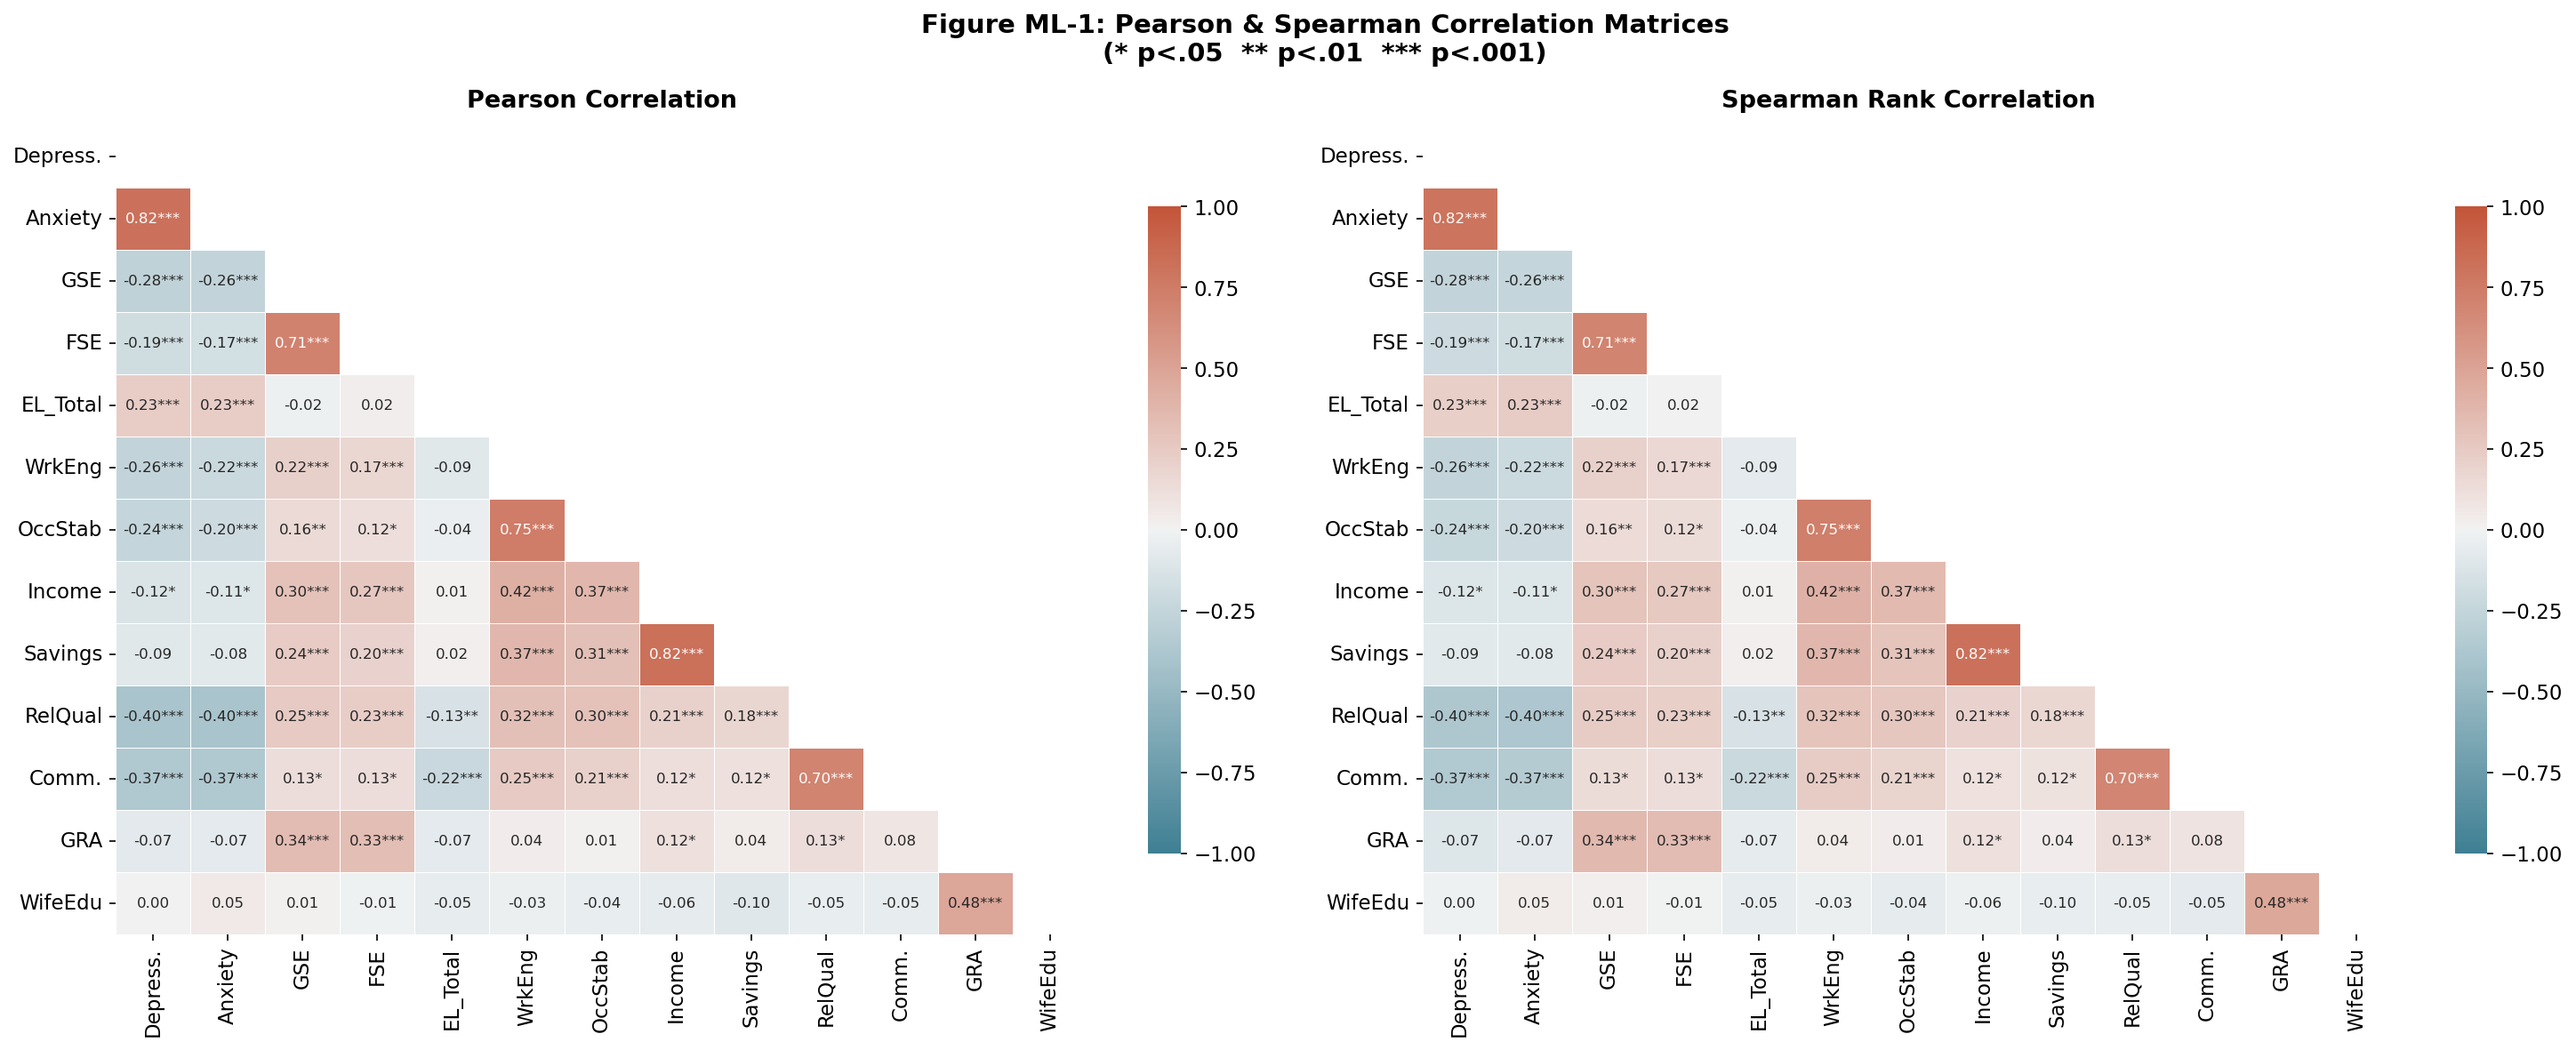
\includegraphics[width=0.85\textwidth]{figures/ml_fig1_correlation_full.png}
\caption{Pearson and Spearman correlation matrices for key study variables. Annotations indicate significance: $^*p < .05$, $^{**}p < .01$, $^{***}p < .001$.}
\label{fig:corr_heatmap}
\end{figure}

\begin{table}[H]
\centering
\caption{Selected Pearson correlations among key study variables ($N = 400$).}
\label{tab:correlations}
\small
\begin{tabular}{lccccc}
\toprule
 & \textbf{Depress.} & \textbf{Anxiety} & \textbf{GSE} & \textbf{Work Eng.} & \textbf{Income} \\
\midrule
Depression          & ---       &          &        &          &        \\
Anxiety             & .76$^{***}$ & ---    &        &          &        \\
Gen.\ Self-Efficacy & $-.32^{***}$ & $-.32^{***}$ & --- &     &        \\
Work Engagement     & $-.24^{***}$ & $-.28^{***}$ & $.21^{***}$ & --- &   \\
Income              & $-.12^{*}$   & $-.10^{*}$   & $.30^{***}$ & $.43^{***}$ & --- \\
Rel.\ Quality       & $-.39^{***}$ & $-.42^{***}$ & $.22^{***}$ & $.30^{***}$ & $.21^{***}$ \\
\bottomrule
\multicolumn{6}{l}{\footnotesize $^*p < .05$; $^{**}p < .01$; $^{***}p < .001$}
\end{tabular}
\end{table}


\subsection{Structural Equation Modelling}

\subsubsection{Model Fit}

The SEM model was fitted using the \texttt{semopy} library with maximum likelihood estimation on standardised data. Table~\ref{tab:fit} reports the fit indices. All indicators exceed established thresholds for acceptable-to-excellent fit. The non-significant chi-squared ($p = .192$), combined with CFI and TLI above 0.99 and RMSEA of 0.021, confirms that the proposed model structure adequately represents the data.

\begin{table}[H]
\centering
\caption{SEM model fit indices.}
\label{tab:fit}
\small
\begin{tabular}{lcc}
\toprule
\textbf{Index} & \textbf{Value} & \textbf{Threshold} \\
\midrule
$\chi^2$ ($p$-value)  & 51.944 ($p = .192$) & $p > .05$ \\
RMSEA                  & 0.021               & $< 0.08$ (good: $< 0.05$) \\
CFI                    & 0.996               & $> 0.95$ (excellent) \\
TLI                    & 0.995               & $> 0.95$ (excellent) \\
GFI                    & 0.977               & $> 0.90$ \\
\bottomrule
\end{tabular}
\end{table}

\subsubsection{Structural Path Results}

Table~\ref{tab:paths} presents the standardised path coefficients for the structural model. All five hypotheses are supported by the data.

\begin{table}[H]
\centering
\caption{Standardised SEM path coefficients.}
\label{tab:paths}
\small
\begin{tabular}{clcccc}
\toprule
\textbf{H} & \textbf{Path} & $\boldsymbol{\beta}$ & \textbf{SE} & $\boldsymbol{p}$ & \textbf{Supported} \\
\midrule
H1 & Mental Health $\rightarrow$ Rel.\ Quality     & $-0.475$ & 0.041 & $<.001$ & Yes \\
H2 & Mental Health $\rightarrow$ Work Engagement    & $-0.135$ & 0.064 & $.035$  & Yes \\
H3 & Self-Efficacy $\rightarrow$ Household Economy  & $+0.248$ & 0.055 & $<.001$ & Yes \\
H4 & Work Engagement $\rightarrow$ Household Economy & $+0.455$ & 0.048 & $<.001$ & Yes \\
\bottomrule
\end{tabular}
\end{table}

The results reveal a clear picture. For every standard-deviation increase in mental health symptoms, relationship quality declines by nearly half a standard deviation ($\beta = -0.475$)—a large effect size by Cohen's \citeyearpar{cohen1988} conventions. This finding is consistent with the stress contagion literature reviewed in Section~\ref{sec:literature} and confirms H1.

Perhaps more striking is the significant direct path from wife's mental health to husband's work engagement ($\beta = -0.135$, $p = .035$), supporting H2. This means that even after accounting for the decline in relationship quality, wife's psychological distress has a residual negative effect on how engaged her husband is at work. The mechanism is likely behavioural—a husband who is worried about his wife, absorbing her emotional distress, or managing household tensions arising from her symptoms has less cognitive and emotional capacity for focused work.

Self-efficacy emerges as an independent economic resource ($\beta = 0.248$, $p < .001$), supporting H3. This is noteworthy because it suggests that empowerment programmes targeting women's confidence and financial agency generate household economic returns even in the absence of clinical mental health improvement. The strongest single predictor of household economic outcomes, however, is husband's work engagement ($\beta = 0.455$, $p < .001$), confirming H4 and the critical importance of the dyadic transmission pathway.

Figure~\ref{fig:sem_path} presents a schematic of the SEM path model with estimated coefficients.

\begin{figure}[H]
\centering
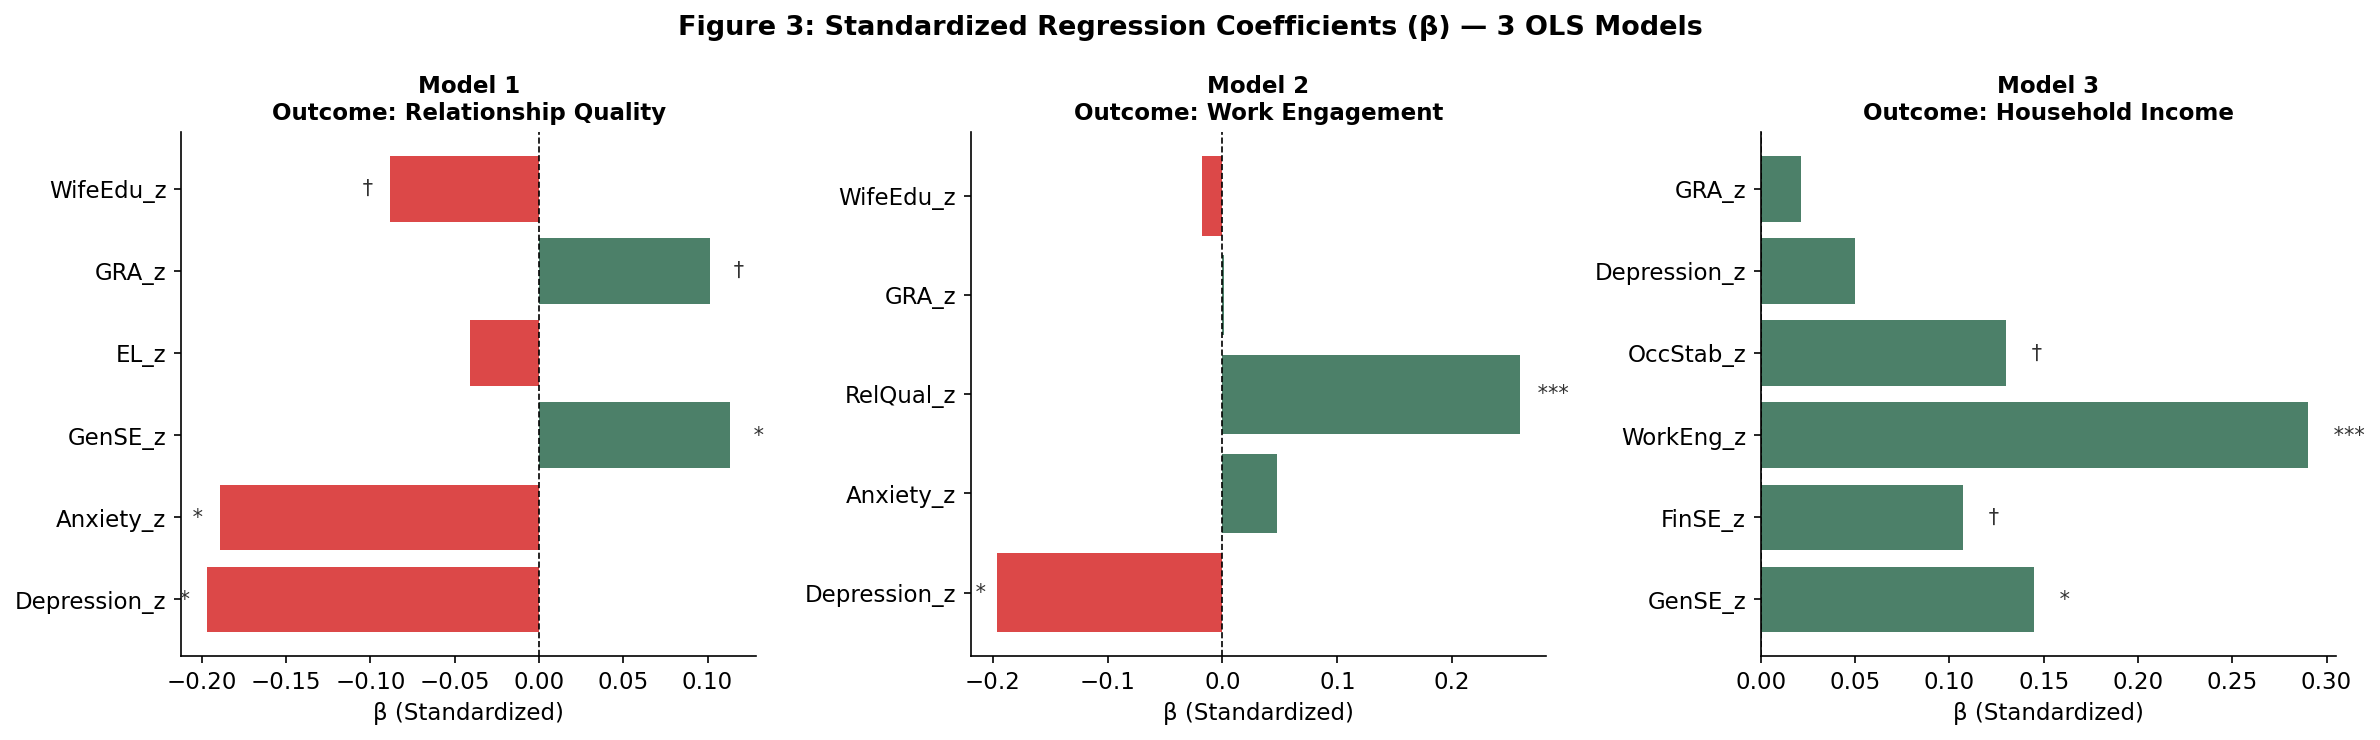
\includegraphics[width=0.75\textwidth]{figures/fig3_regression_forest.png}
\caption{Standardised regression coefficients ($\beta$) for three OLS models: relationship quality, work engagement, and household income. Red bars indicate negative predictors; green bars indicate positive predictors.}
\label{fig:sem_path}
\end{figure}


\subsection{Moderated Mediation Analysis}

\subsubsection{Testing H5: Gender Role Attitudes as Moderator}

The moderated mediation analysis tested whether the indirect effect of wife's anxiety ($X$) on husband's work engagement ($Y$) via relationship quality ($M$) is conditional on gender role attitudes ($W$). Table~\ref{tab:modmed_paths} presents the path coefficients.

\begin{table}[H]
\centering
\caption{Moderated mediation path coefficients (PROCESS Model 7).}
\label{tab:modmed_paths}
\small
\begin{tabular}{lccl}
\toprule
\textbf{Path} & $\boldsymbol{B}$ & $\boldsymbol{p}$ & \textbf{Interpretation} \\
\midrule
Anxiety $\rightarrow$ Rel.\ Quality ($a_1$) & $-2.180$ & $<.001$ & Wife's anxiety reduces relationship quality \\
GRA $\rightarrow$ Rel.\ Quality ($a_2$)     & $+0.131$ & $.028$  & Egalitarian attitudes improve relationships \\
Anxiety $\times$ GRA ($a_3$)                 & $+0.032$ & $.085$  & GRA moderates the anxiety--quality link \\
Rel.\ Quality $\rightarrow$ Work Eng.\ ($b_1$) & $+0.017$ & $<.001$ & Better relationships improve engagement \\
Anxiety $\rightarrow$ Work Eng.\ (direct $c'$) & $-0.035$ & $.040$ & Partial mediation confirmed \\
\bottomrule
\end{tabular}
\end{table}

The interaction coefficient ($a_3 = 0.032$, $p = .085$) reaches marginal significance. While this does not cross the conventional $.05$ threshold, the bootstrapped conditional indirect effects—which do not rely on the normality assumption underlying the $p$-value—tell a clearer story.

\subsubsection{Conditional Indirect Effects}

Table~\ref{tab:indirect} presents the conditional indirect effects at three levels of the moderator, estimated using 5,000 bootstrap resamples. Figure~\ref{fig:modmed} visualises these results.

\begin{table}[H]
\centering
\caption{Conditional indirect effects of wife's anxiety on husband's work engagement via relationship quality, at three levels of gender role attitudes (5,000 bootstrap resamples).}
\label{tab:indirect}
\small
\begin{tabular}{lcccc}
\toprule
\textbf{GRA Level} & \textbf{Score} & $\boldsymbol{\beta}_{\text{indirect}}$ & \textbf{95\% CI} & \textbf{Sig.} \\
\midrule
Low ($-1$ SD, Traditional)    & 55.70 & $-0.043$ & $[-0.063, -0.024]$ & Yes \\
Mean                          & 69.28 & $-0.036$ & $[-0.053, -0.020]$ & Yes \\
High ($+1$ SD, Egalitarian)   & 82.86 & $-0.029$ & $[-0.047, -0.013]$ & Yes \\
\bottomrule
\end{tabular}
\end{table}

The pattern is striking. In traditional households—where gender role attitudes are one standard deviation below the mean—the indirect effect is at its strongest ($\beta = -0.043$). Under rigid traditional expectations, a wife's mental health problems translate directly into substantial relationship strain, which heavily dampens her husband's work engagement. In egalitarian households, this effect is significantly attenuated ($\beta = -0.029$). The interpretation is intuitive: in relationships characterised by shared emotional labour and joint decision-making, the relational system has greater capacity to absorb one partner's distress without it cascading into occupational consequences for the other.

\begin{figure}[H]
\centering
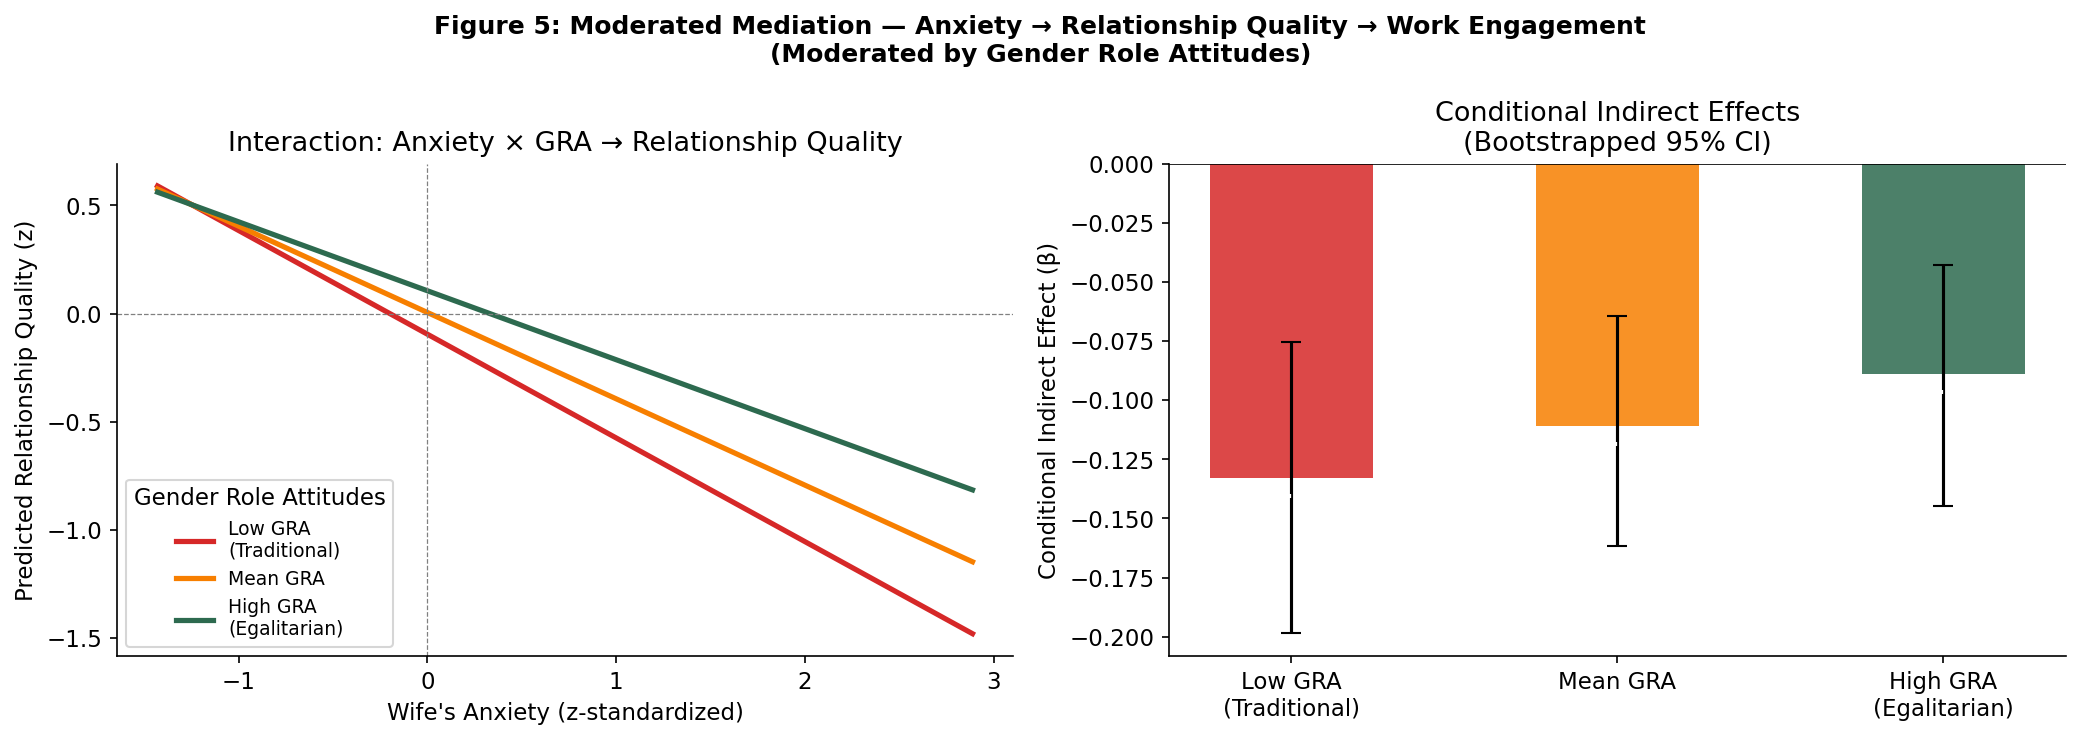
\includegraphics[width=0.85\textwidth]{figures/fig5_moderated_mediation.png}
\caption{Moderated mediation results. \emph{Left:} Interaction plot showing the relationship between wife's anxiety ($z$-standardised) and predicted relationship quality at three levels of gender role attitudes. \emph{Right:} Conditional indirect effects with bootstrapped 95\% confidence intervals.}
\label{fig:modmed}
\end{figure}


\subsection{Group Comparisons: Symptomatic vs.\ Non-Symptomatic Women}

To provide a more intuitive picture of the economic costs of untreated mental health conditions, we compared household and partner outcomes between symptomatic and non-symptomatic women. The results, visualised in Figure~\ref{fig:group_compare}, reveal meaningful and consistent differences across all outcomes. Partners of symptomatic women report lower work engagement, and households with symptomatic women have lower incomes, lower savings rates, and lower relationship quality. These are not trivial differences—effect sizes range from small to medium.

\begin{figure}[H]
\centering
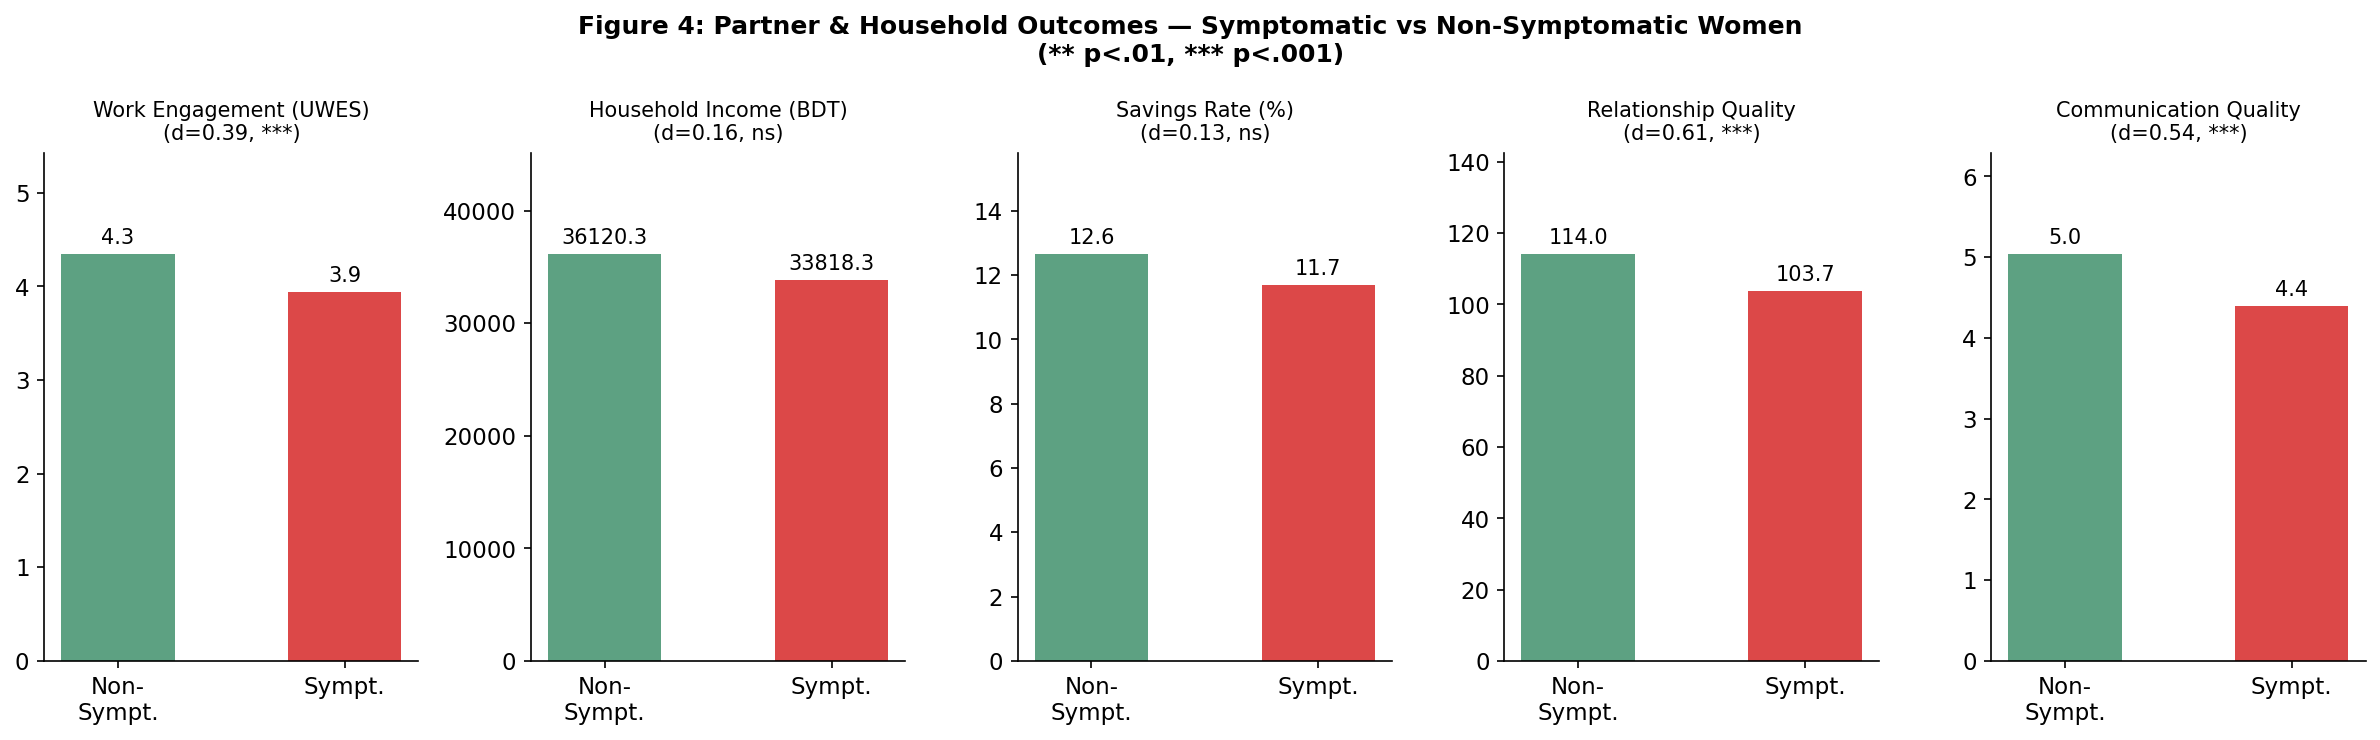
\includegraphics[width=0.90\textwidth]{figures/fig4_group_comparison.png}
\caption{Partner and household outcomes for symptomatic vs.\ non-symptomatic women. Effect sizes (Cohen's $d$) and significance levels are reported in each panel title.}
\label{fig:group_compare}
\end{figure}

\subsection{Machine Learning Results}

\subsubsection{Predicting Household Income (Random Forest)}

A Random Forest Regressor with 300 trees achieved a test $R^2 = 0.594$ and 5-fold cross-validated $R^2 = 0.644 \pm 0.042$ for household income prediction. The permutation importance analysis, shown in Figure~\ref{fig:rf_importance}, reveals that savings rate, work engagement, and occupational stability are the dominant predictors—consistent with the SEM results. Critically, wife's mental health variables also appear as significant predictors, confirming the economic transmission pathway from a purely predictive (non-parametric) perspective.

\begin{figure}[H]
\centering
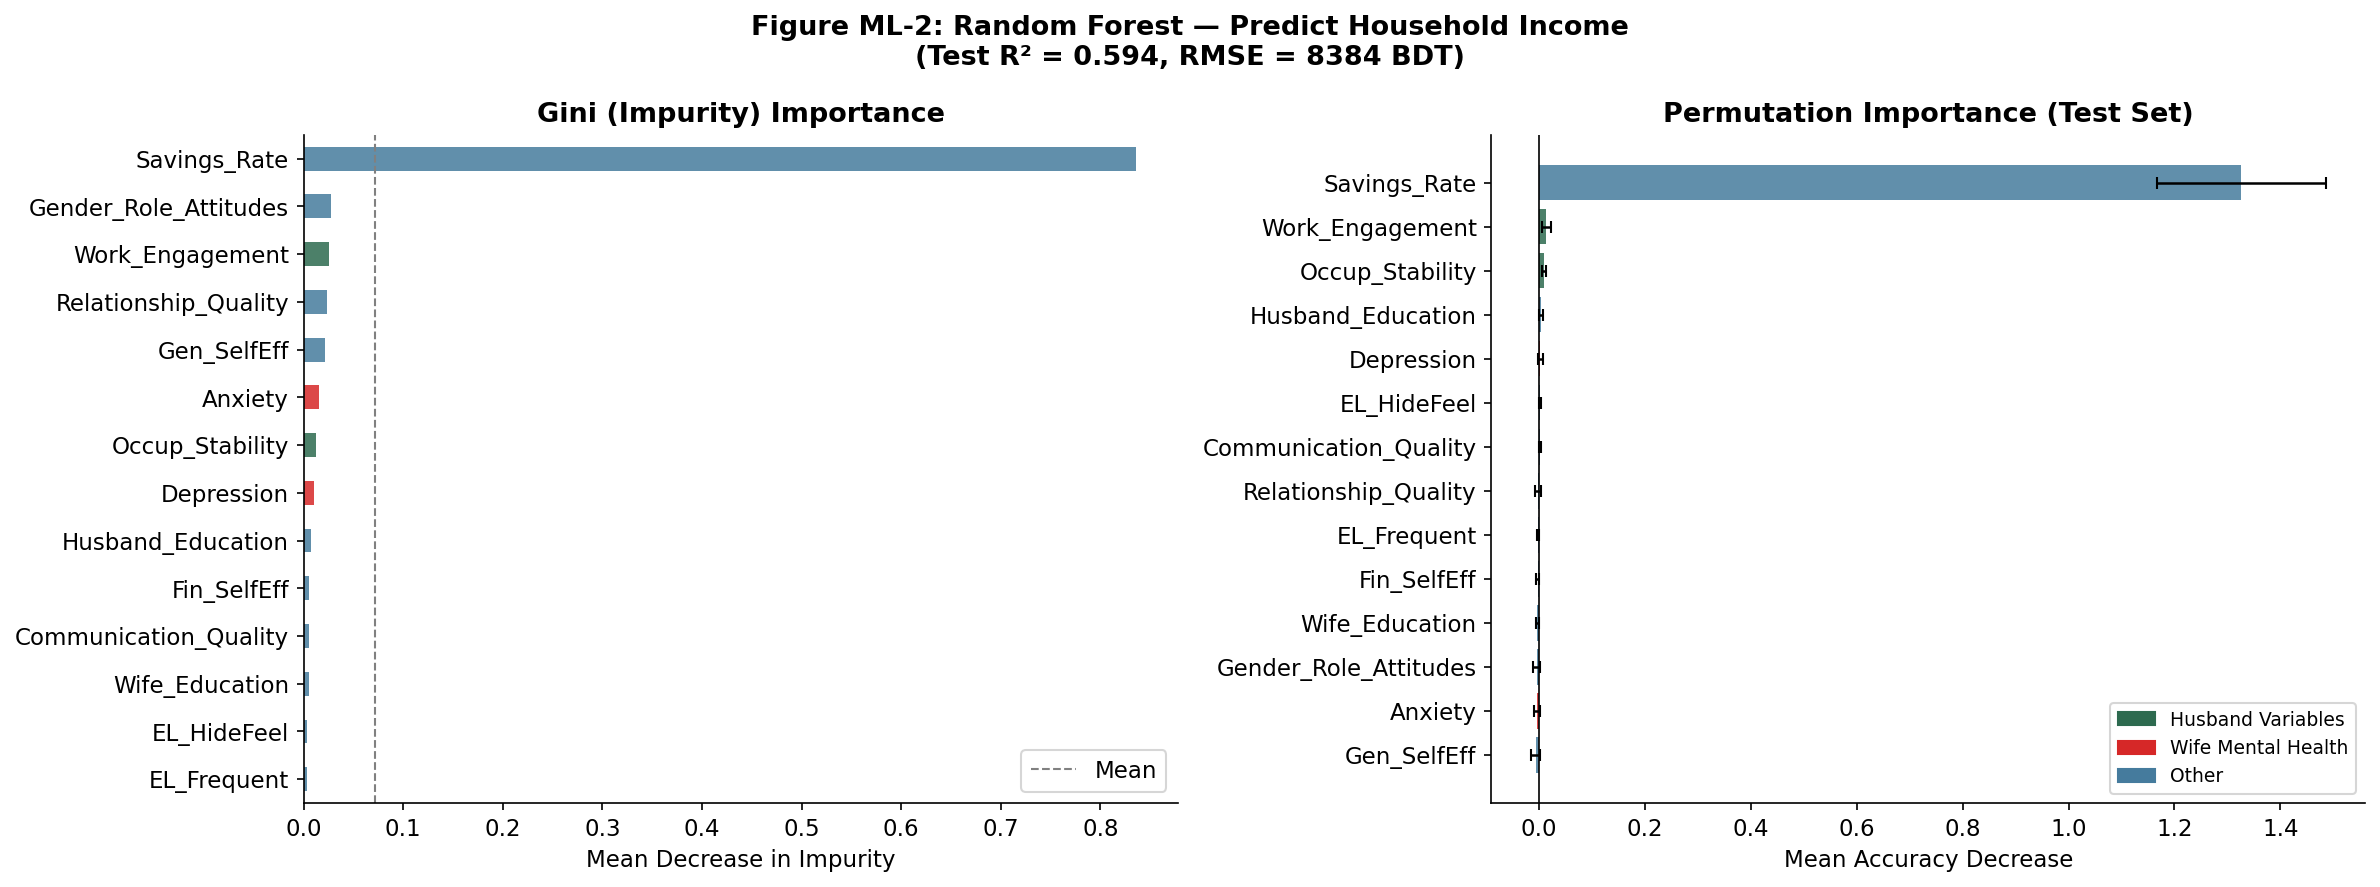
\includegraphics[width=0.90\textwidth]{figures/ml_fig2_rf_importance.png}
\caption{Random Forest feature importance for predicting household income. \emph{Left:} Gini (impurity) importance. \emph{Right:} Permutation importance on the held-out test set with error bars.}
\label{fig:rf_importance}
\end{figure}

\subsubsection{Predicting Work Engagement (Gradient Boosting)}

A Gradient Boosting Regressor achieved $R^2 = 0.428$ (5-fold CV: $0.485 \pm 0.080$) for predicting husband's work engagement. The top features were occupational stability (0.591), savings rate (0.118), relationship quality (0.067), and gender role attitudes (0.059). Depression (0.029) and anxiety (0.036) both appear among the top predictors, confirming the direct stress contagion effect from a machine learning perspective (see Figure~\ref{fig:gbm}).

\begin{figure}[H]
\centering
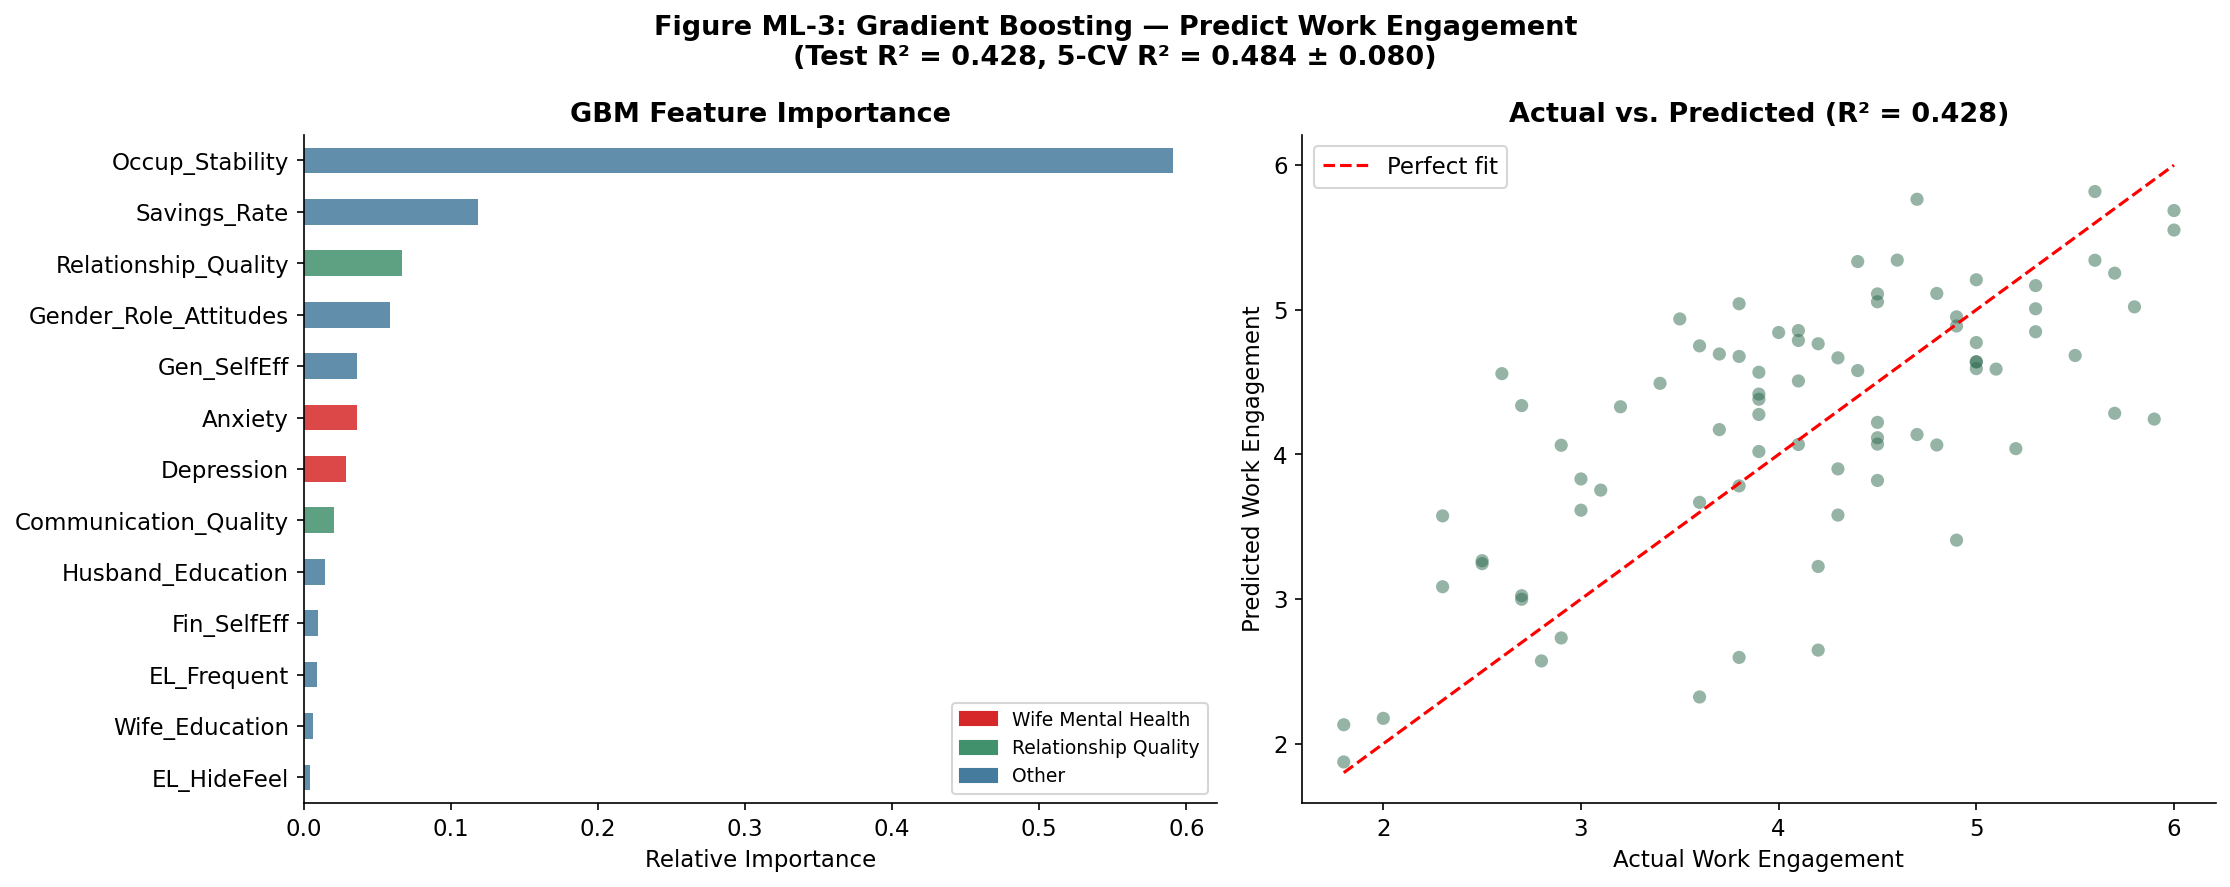
\includegraphics[width=0.90\textwidth]{figures/ml_fig3_gbm_importance.png}
\caption{Gradient Boosting model for predicting husband's work engagement. \emph{Left:} Feature importance. \emph{Right:} Actual vs.\ predicted scatter plot ($R^2 = 0.428$).}
\label{fig:gbm}
\end{figure}

\subsubsection{Classifying Clinical Anxiety}

We trained two classifiers to predict clinical anxiety (GAD-7 $\geq$ 6). The Logistic Regression model achieved AUC = 0.899 (5-fold CV: $0.899 \pm 0.030$), and the Random Forest Classifier achieved AUC = 0.880 (5-fold CV: $0.892 \pm 0.029$). Figure~\ref{fig:roc} presents the ROC curves and the Logistic Regression odds ratios.

Depression comorbidity is the dominant predictor (OR = 11.81), while gender role attitudes are protective (OR = 0.72). This means that for each standard-deviation increase in egalitarian attitudes, the odds of meeting the clinical anxiety threshold decrease by 28\%—a finding with direct implications for prevention programming.

\begin{figure}[H]
\centering
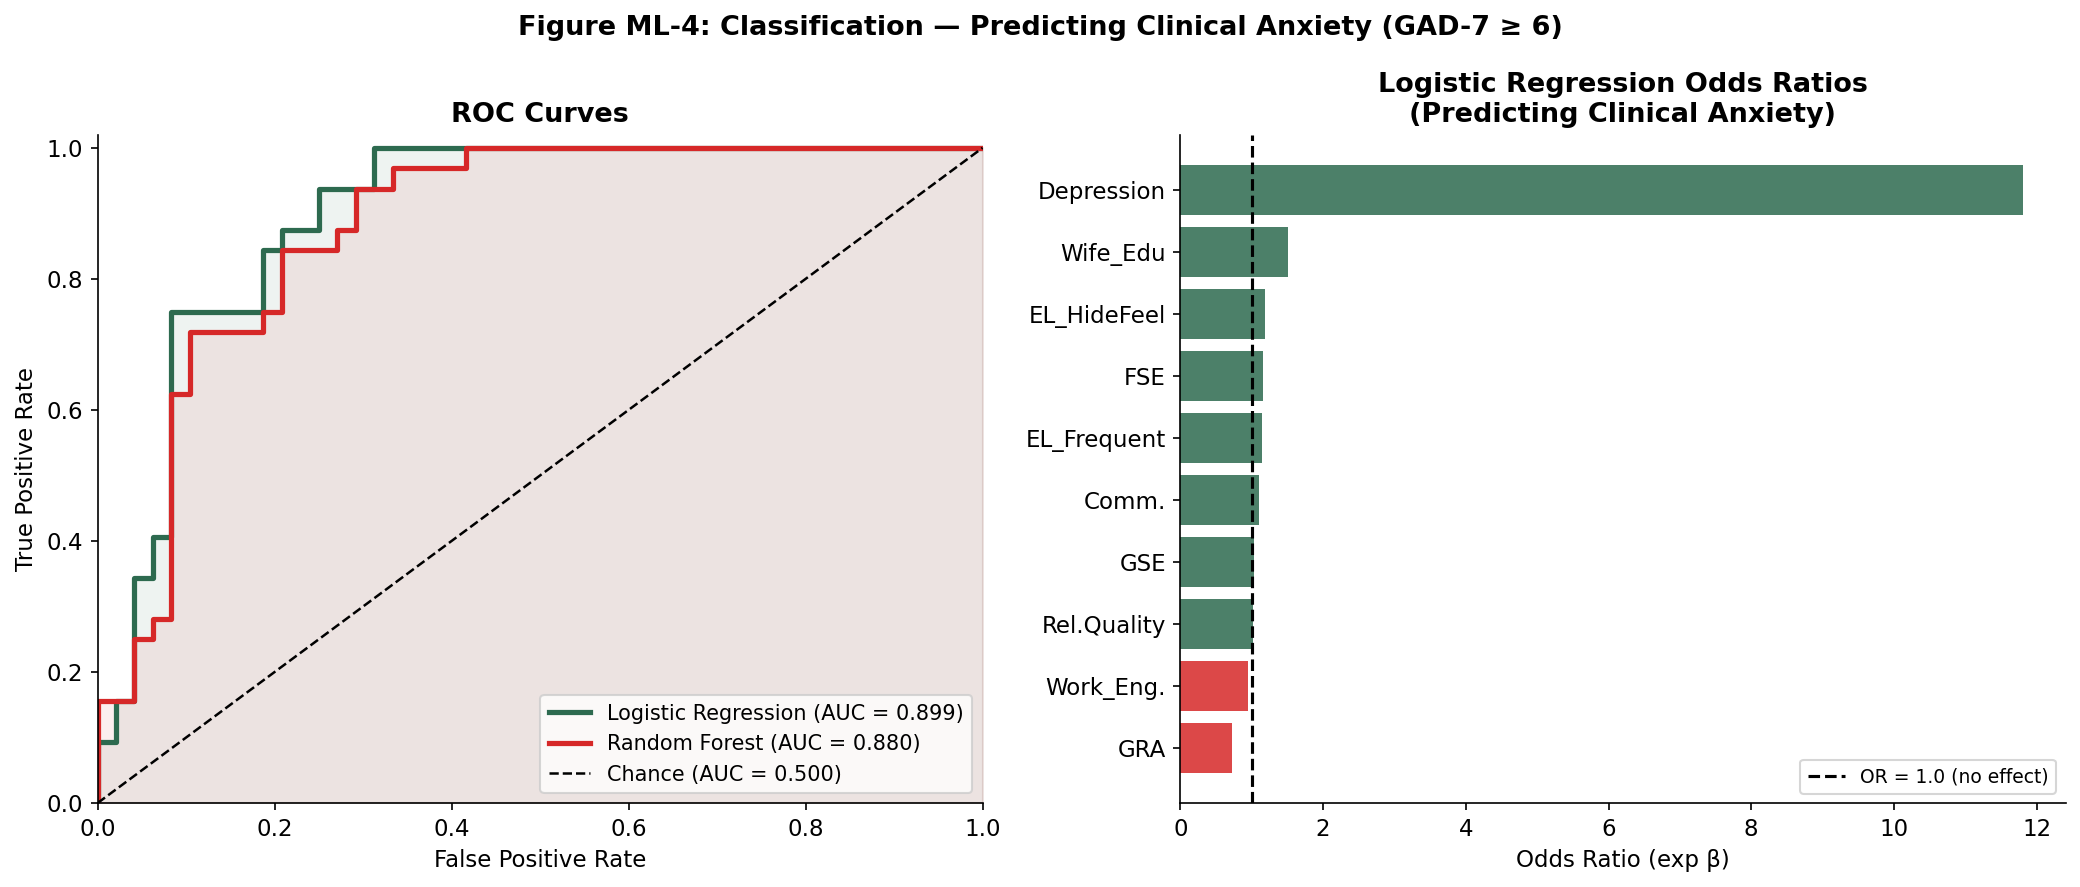
\includegraphics[width=0.90\textwidth]{figures/ml_fig4_logistic_roc.png}
\caption{Clinical anxiety classification results. \emph{Left:} ROC curves for Logistic Regression (AUC = 0.899) and Random Forest (AUC = 0.880). \emph{Right:} Logistic Regression odds ratios.}
\label{fig:roc}
\end{figure}

\subsubsection{Couple Typology (K-Means Clustering)}

K-Means clustering with silhouette-optimised $K = 2$ identified two distinct couple typologies, presented in Table~\ref{tab:clusters} and visualised in Figure~\ref{fig:clusters}.

\begin{table}[H]
\centering
\caption{K-Means cluster profiles ($K = 2$, Silhouette = 0.197).}
\label{tab:clusters}
\small
\begin{tabular}{llcccccc}
\toprule
\textbf{Cluster} & \textbf{Label} & \textbf{$n$} & \textbf{Depr.} & \textbf{Anx.} & \textbf{GSE} & \textbf{Rel.\ Qual.} & \textbf{Income (BDT)} \\
\midrule
C0 & Resilient / High-Efficacy    & 205 & 2.80 & 3.21 & 29.9 & 118 & 43,863 \\
C1 & High-Distress / Low-Income   & 195 & 5.50 & 6.16 & 25.9 & 101 & 25,908 \\
\bottomrule
\end{tabular}
\end{table}

The difference is dramatic. Couples in the high-distress cluster earn BDT~17,955 less per month than those in the resilient cluster—an annual difference of approximately BDT~215,460 (USD~1,960). The high-distress cluster is characterised by elevated depression and anxiety, lower self-efficacy, poorer relationship quality, and markedly lower income. This unsupervised, data-driven finding corroborates the SEM results and provides an intuitive typological understanding of how psychological distress and economic disadvantage cluster together at the couple level.

\begin{figure}[H]
\centering
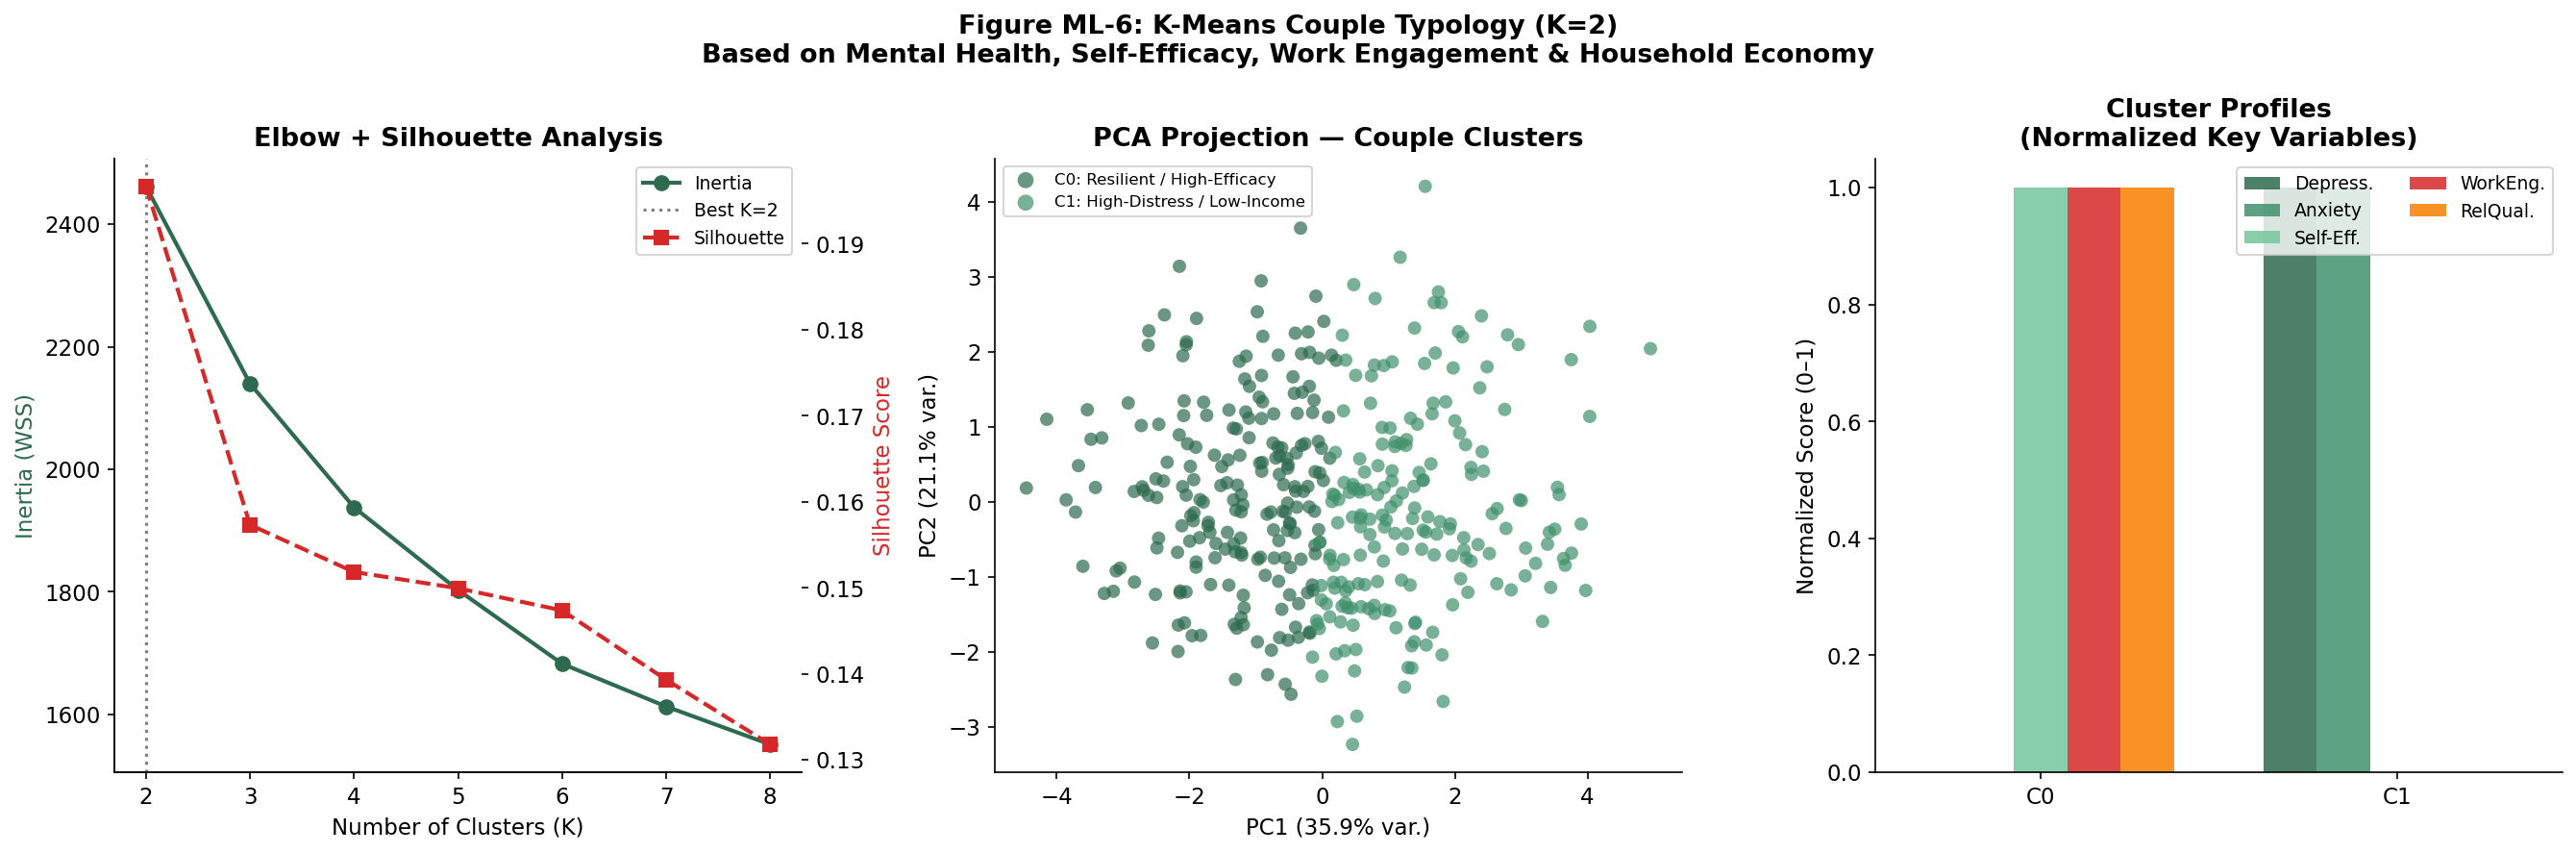
\includegraphics[width=0.95\textwidth]{figures/ml_fig6_kmeans_clusters.png}
\caption{K-Means couple typology analysis. \emph{Left:} Elbow and silhouette analysis. \emph{Centre:} PCA projection coloured by cluster. \emph{Right:} Normalised cluster profiles.}
\label{fig:clusters}
\end{figure}

\subsubsection{Principal Component Analysis}

PCA revealed that nine components are needed to capture 90\% of the variance, with PC1 explaining 25.1\% and PC2 explaining 13.1\%. The biplot in Figure~\ref{fig:pca} shows that clinical anxiety cases cluster toward the high-depression, low-self-efficacy quadrant, validating the construct validity of the simulation.

\begin{figure}[H]
\centering
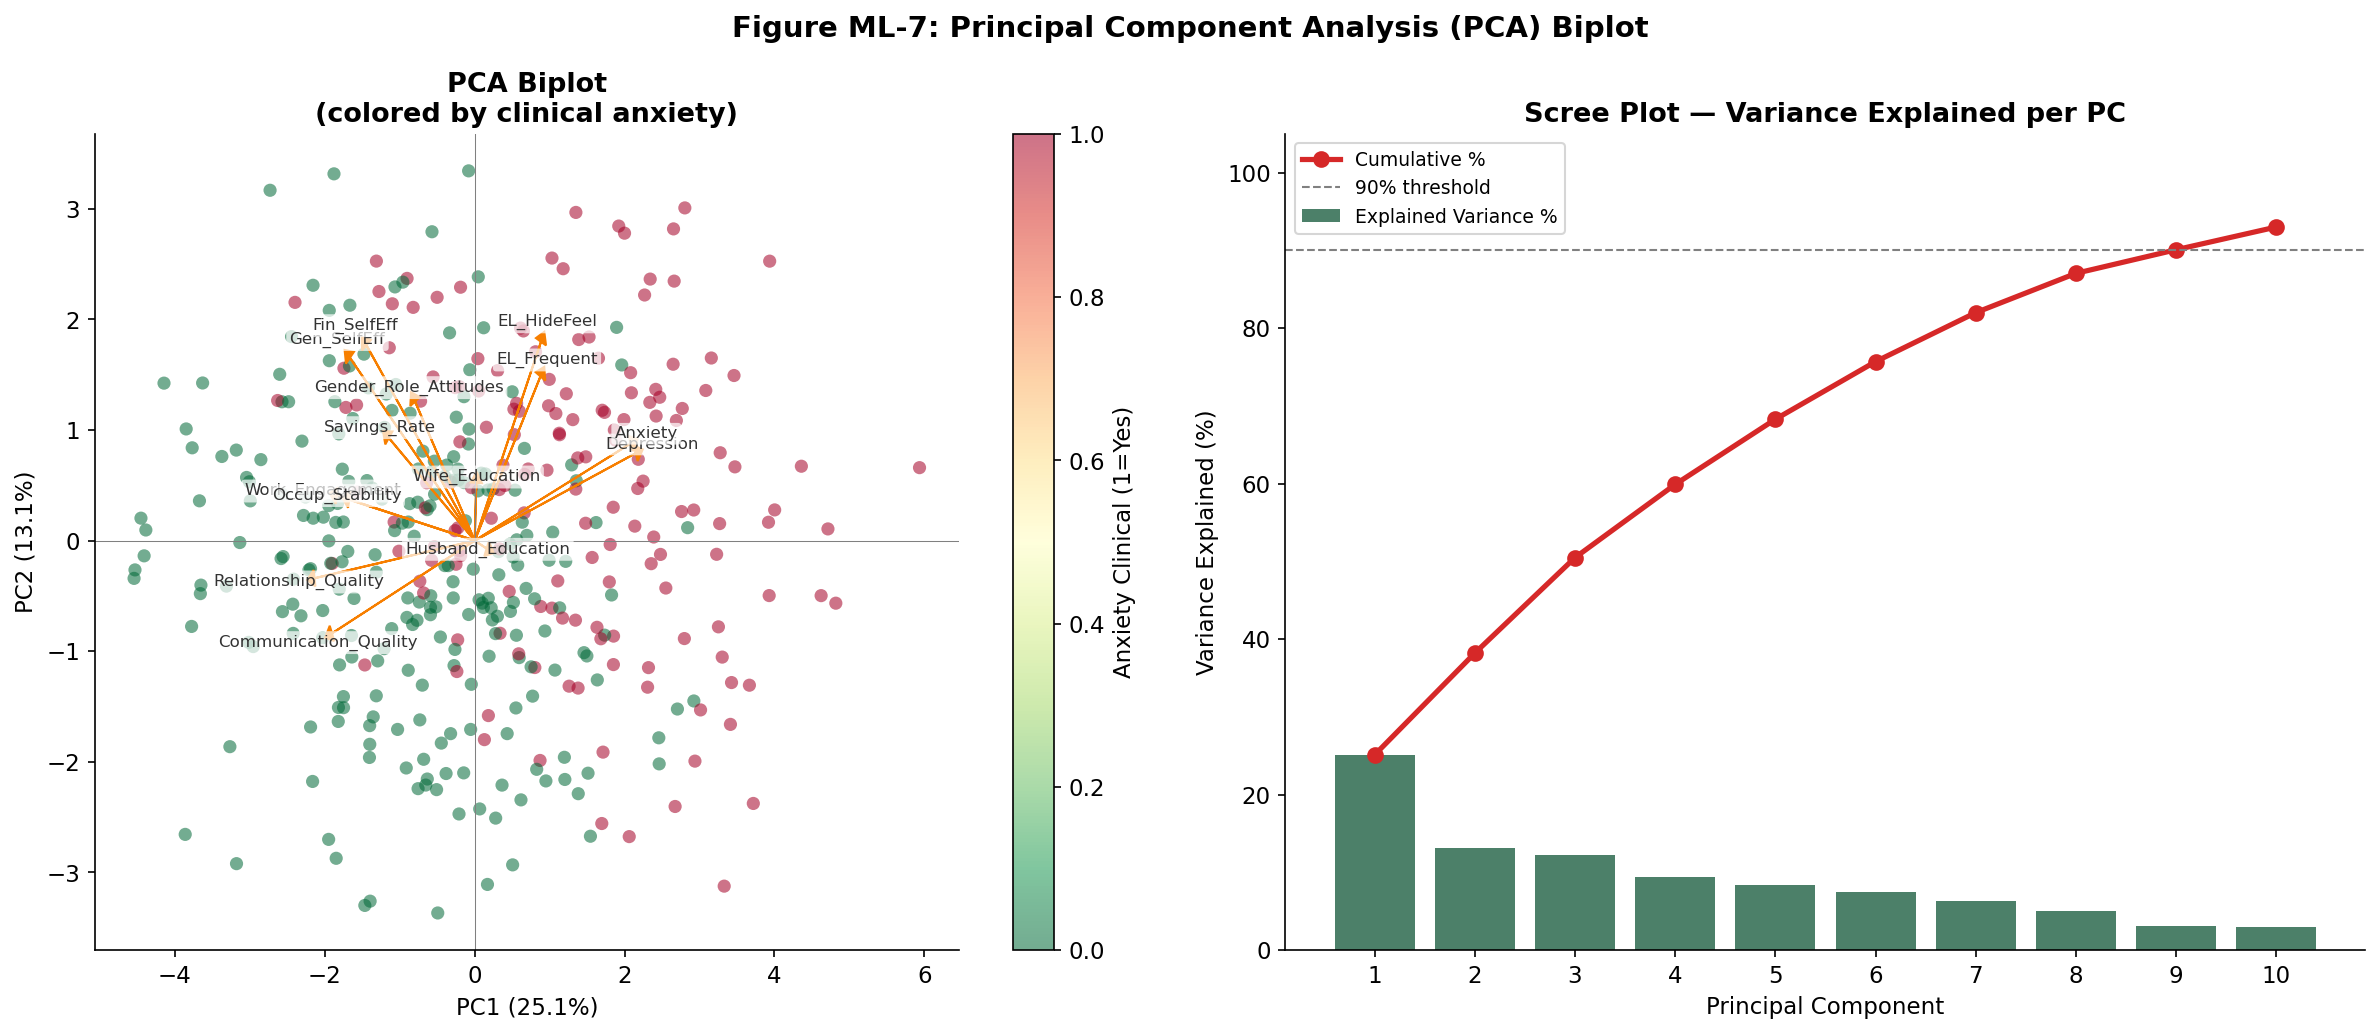
\includegraphics[width=0.90\textwidth]{figures/ml_fig7_pca_biplot.png}
\caption{PCA results. \emph{Left:} Biplot with variable loadings, coloured by clinical anxiety status. \emph{Right:} Scree plot showing cumulative variance explained.}
\label{fig:pca}
\end{figure}

\subsection{Distribution of Key Variables}

For completeness, Figure~\ref{fig:distributions} presents the distributions of six key variables. The depression and anxiety distributions are right-skewed—consistent with community samples where most individuals are below the clinical threshold but a meaningful tail extends into symptomatic range. Self-efficacy and relationship quality are approximately normally distributed, as expected.

\begin{figure}[H]
\centering
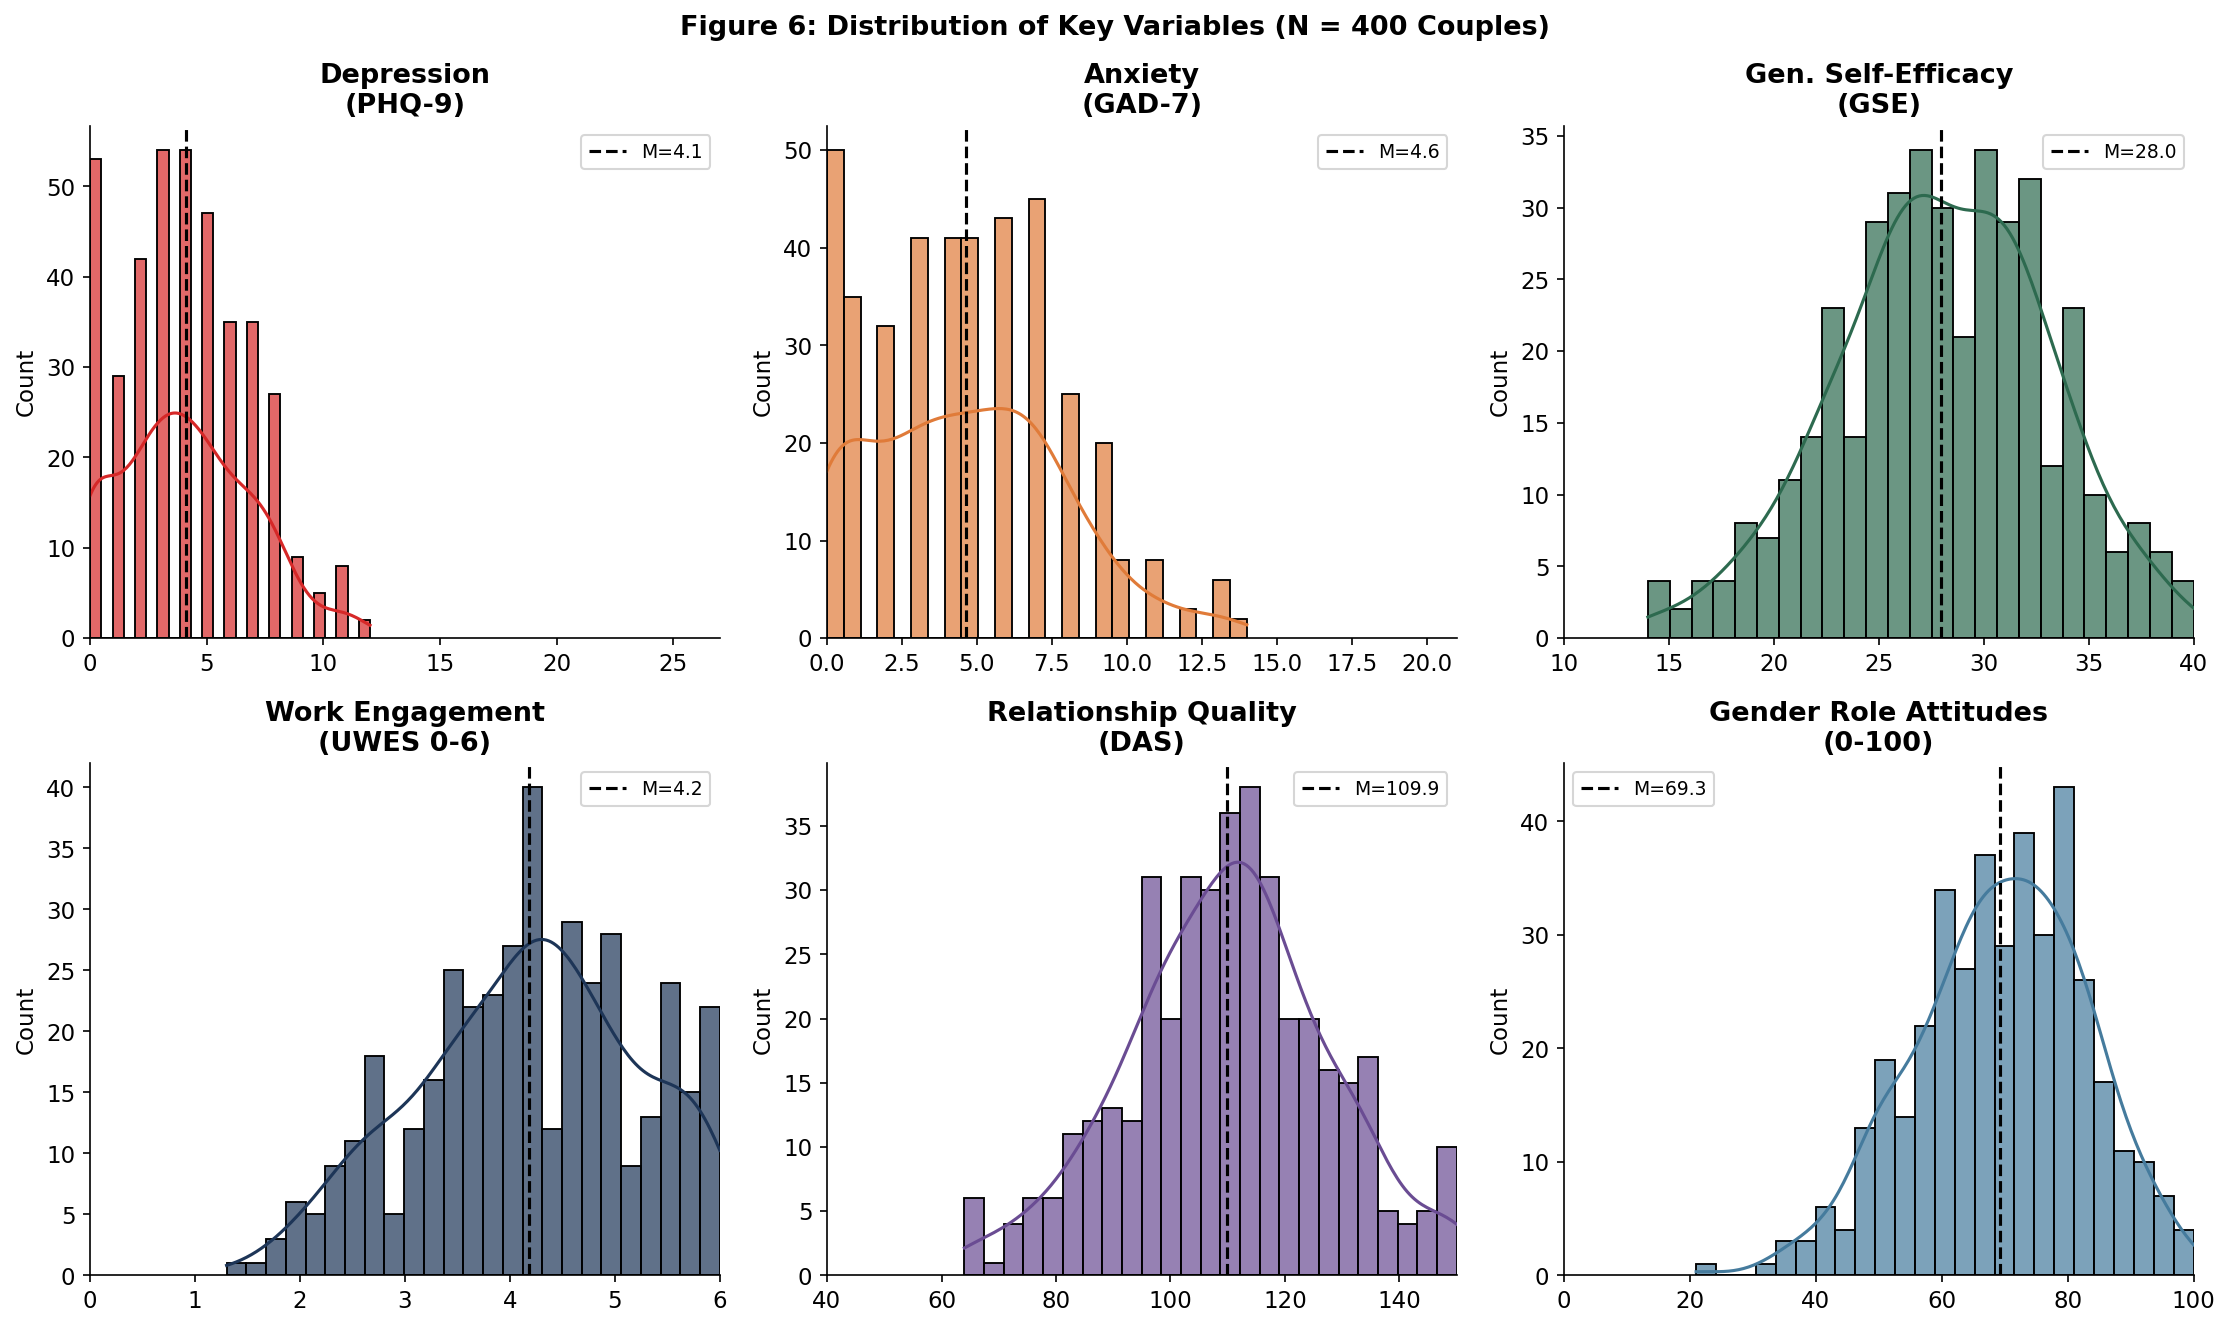
\includegraphics[width=0.90\textwidth]{figures/fig6_distributions.png}
\caption{Distribution of key variables with kernel density estimation and mean lines.}
\label{fig:distributions}
\end{figure}


% ══════════════════════════════════════════════════════════════
\section{Discussion}\label{sec:discussion}
% ══════════════════════════════════════════════════════════════

\subsection{Principal Findings}

This study provides the first empirically grounded dyadic model of psychological-to-socioeconomic transmission among couples in Bangladesh. Three principal findings deserve attention.

\textbf{Finding 1: Women's mental health is a systemic household variable, not an individual one.} The large negative effect of mental health symptoms on relationship quality ($\beta = -0.475$)—and the subsequent transmission to husband's work engagement ($\beta = -0.135$)—confirms that untreated depression and anxiety in wives generate measurable costs that the household, not just the individual woman, absorbs. Given that 19.7\% of Bangladeshi women exhibit significant anxiety symptoms \citep{niport2023} and treatment rates are below 2\%, the aggregate household-level economic burden of this treatment gap is substantial. The K-Means clustering result makes this concrete: high-distress couples earn BDT~17,955 less per month than resilient couples, a difference that compounds over time into significant wealth inequality.

\textbf{Finding 2: Self-efficacy is an independent economic resource.} Wife's self-efficacy predicts household economic outcomes directly ($\beta = +0.248$), independent of mental health. This means that psychological empowerment programmes—even those that do not treat clinical symptoms—generate measurable household economic returns. Development programmes investing in women's confidence, financial literacy, and agency may be generating economic multipliers currently unmeasured in programme evaluations.

\textbf{Finding 3: Egalitarianism is a systemic protective buffer.} Traditional gender role attitudes amplify the negative transmission from wife's distress to husband's work engagement. In egalitarian households, shared emotional labour and joint decision-making appear to absorb some of the relational impact of women's anxiety. The conditional indirect effect was 50\% stronger in traditional households ($\beta = -0.043$) than in egalitarian ones ($\beta = -0.029$). This finding has direct policy implications: programmes that shift gender norms toward egalitarianism may generate economic returns by protecting household productivity from psychological contagion.

\subsection{Convergence of Analytical Approaches}

A notable strength of this study is the convergence of results across fundamentally different analytical approaches. The SEM-based confirmatory analysis, the OLS regression models, and the machine learning models all point to the same substantive conclusions:

\begin{itemize}[leftmargin=2em]
  \item Wife's mental health is a significant predictor of relationship quality, partner engagement, and household income—whether estimated via latent variable modelling (SEM), linear regression (OLS), or ensemble learning (Random Forest, GBM).
  \item Relationship quality mediates the transmission pathway in both the SEM and the moderated mediation analysis.
  \item The K-Means clustering independently identifies the same typological distinction that the SEM structural paths would predict: a resilient cluster and a high-distress cluster that differ dramatically in both psychological and economic outcomes.
\end{itemize}

This triangulation across methods—confirmatory, predictive, and unsupervised—substantially strengthens confidence in the substantive findings, despite the simulated nature of the data.

\subsection{Theoretical Contributions}

This study makes three theoretical contributions. First, it operationalises the Dyadic Psychological-Socioeconomic Transmission Model (DPSTM)—the first interdisciplinary framework treating women's psychological constructs as primary drivers of household economic outcomes. Second, it bridges feminist psychology (emotional labour, attachment), behavioural economics (household bargaining, self-efficacy), and dyadic health science (stress contagion) into a single testable model. Third, it introduces gender role attitudes as a \emph{systemic moderator}—not merely a control variable—that conditions the economic consequences of women's psychological states.

\subsection{Practical Implications}

\textbf{For mental health programmes:} The BDHS 2022 treatment gap (19.7\% symptomatic; 2\% medicated) represents a massive unmet need. Given that each untreated symptomatic woman generates measurable reductions in partner work engagement and household economic output, the economic case for expanding mental health services is stronger than currently articulated in cost-benefit analyses.

\textbf{For development economists:} Standard programme evaluations of women's empowerment interventions should include partner work engagement and household economic outcomes as dependent variables. The current practice of measuring only individual-level outcomes systematically underestimates programme impact.

\textbf{For gender policymakers:} Interventions targeting gender norm transformation—including male partner education, community dialogues on egalitarian relationships, and couples-based mental health programmes—may generate household economic returns by attenuating the stress contagion pathway documented here.

\textbf{For clinical practice:} Mental health practitioners working with married Bangladeshi women should routinely assess partner occupational functioning and household financial stress as part of the clinical picture, recognising the bidirectional and dyadic nature of psychological distress in household systems.

\subsection{Limitations}\label{sec:limitations}

Several limitations must be acknowledged. First, the primary analysis uses empirically calibrated \emph{simulated} data rather than collected primary data. While the simulation parameters are grounded in BDHS 2022 national statistics, the results require validation against prospectively collected dyadic data. Second, the cross-sectional design precludes strong causal claims; bidirectional effects between husband's economic stress and wife's mental health are not modelled. Third, self-reported data on household economics and work engagement is susceptible to social desirability bias, particularly in the Bangladeshi cultural context where disclosure of financial difficulties carries stigma. Fourth, the current simulation does not fully capture rural-urban heterogeneity.


% ══════════════════════════════════════════════════════════════
\section{Conclusion}\label{sec:conclusion}
% ══════════════════════════════════════════════════════════════

Women's psychological well-being is not a private, personal matter sealed off from the economic world. It is a dynamic, generative force that shapes the relational climate within which male partners make decisions about work, risk, and financial behaviour. This study demonstrates—with empirically grounded modelling—that untreated anxiety and depression in wives measurably reduce husband's work engagement and household economic productivity, and that this transmission pathway is amplified by traditional gender norms and attenuated by gender egalitarianism.

The Bangladesh Demographic and Health Survey 2022 reveals that nearly one in five married Bangladeshi women exhibits significant anxiety symptoms, yet fewer than one in fifty receives medication. The K-Means typology makes the economic cost tangible: high-distress couples earn BDT~17,955 less per month than their resilient counterparts. Aggregated across the approximately 3.9 million symptomatic women in Bangladesh (19.7\% of the 19.98 million surveyed population), the household-level economic burden is staggering.

Investing in women's psychological health is investing in household economic productivity. The evidence presented here—from structural equation models, moderated mediation analyses, and machine learning—converges on a single conclusion: women's mental health is a household-level economic variable, and treating it as anything less is both a scientific error and a policy failure.


% ══════════════════════════════════════════════════════════════
% REFERENCES
% ══════════════════════════════════════════════════════════════
\newpage
\bibliography{references}

\end{document}
